\documentclass{jfm}
\usepackage{graphicx}
\usepackage{epstopdf, epsfig}
\usepackage{lipsum}
\usepackage{gensymb}
\usepackage{booktabs}
\usepackage{makecell}
\usepackage{multirow}
\usepackage{float}
\usepackage{color}
\usepackage{tikz}
\usetikzlibrary{shapes}
\usepackage{amsmath}
\shorttitle{Genesis of liquid chain}
\shortauthor{V. Sanjay and A. K. Das}
\title{Genesis of Liquid Chain by Collision of Two Laminar Jets}
\author{Vatsal Sanjay,
  Arup K. Das\corresp{\email{arupdas80@gmail.com}}}
\affiliation{Department of Mechanical and Industrial Engineering, Indian Institute of Technology, Roorkee}

\begin{document}
\newcommand{\MarkerCircleRed}{\raisebox{0.5pt}{\tikz{\node[draw,scale=0.4,circle,fill=red!100!red](){};}}}
\newcommand{\MarkerSquareRed}{\raisebox{0.5pt}{\tikz{\node[draw,scale=0.4,regular polygon, regular polygon sides=4,fill=black!20!red](){};}}}
\newcommand{\MarkerDiamondBlack}{\raisebox{0pt}{\tikz{\node[draw,scale=0.4,diamond,fill=black!100!](){};}}}
\newcommand{\MarkerSquareEmpty}{\raisebox{0pt}{\tikz{\node[draw,scale=0.4,regular polygon, regular polygon sides=4](){};}}}
\newcommand{\MarkerCircleEmpty}{\raisebox{0pt}{\tikz{\node[draw,scale=0.4,circle](){};}}}
\maketitle
\begin{abstract}
\end{abstract}
The collision of liquid jets and formation of a sheet in the median plane is illustrated numerically, which subsequently transforms into a chain like fluidic structure with successive dwarf links in mutually orthogonal planes. Flow kinematics is studied with self-similar velocity profile and streamlines to understand the behavior of fluid parcels inside the chain. With the numerical analysis over a wide range of operating parameters, a correlation has been proposed to predict the shape of the links in the chain. Citing analogy between the impact of rims for the formation of elemental links and traversal of damped billiard balls after the collision, an attempt has been made to understand the fundamental physics of the problem through force balance. Finally, the formation of higher order links is proposed as equivalent to the collision between jets of reduced strengths and smaller impingement angles.
\begin{keywords}
\end{keywords}
\section{Introduction}
\begin{figure}
	\centering
	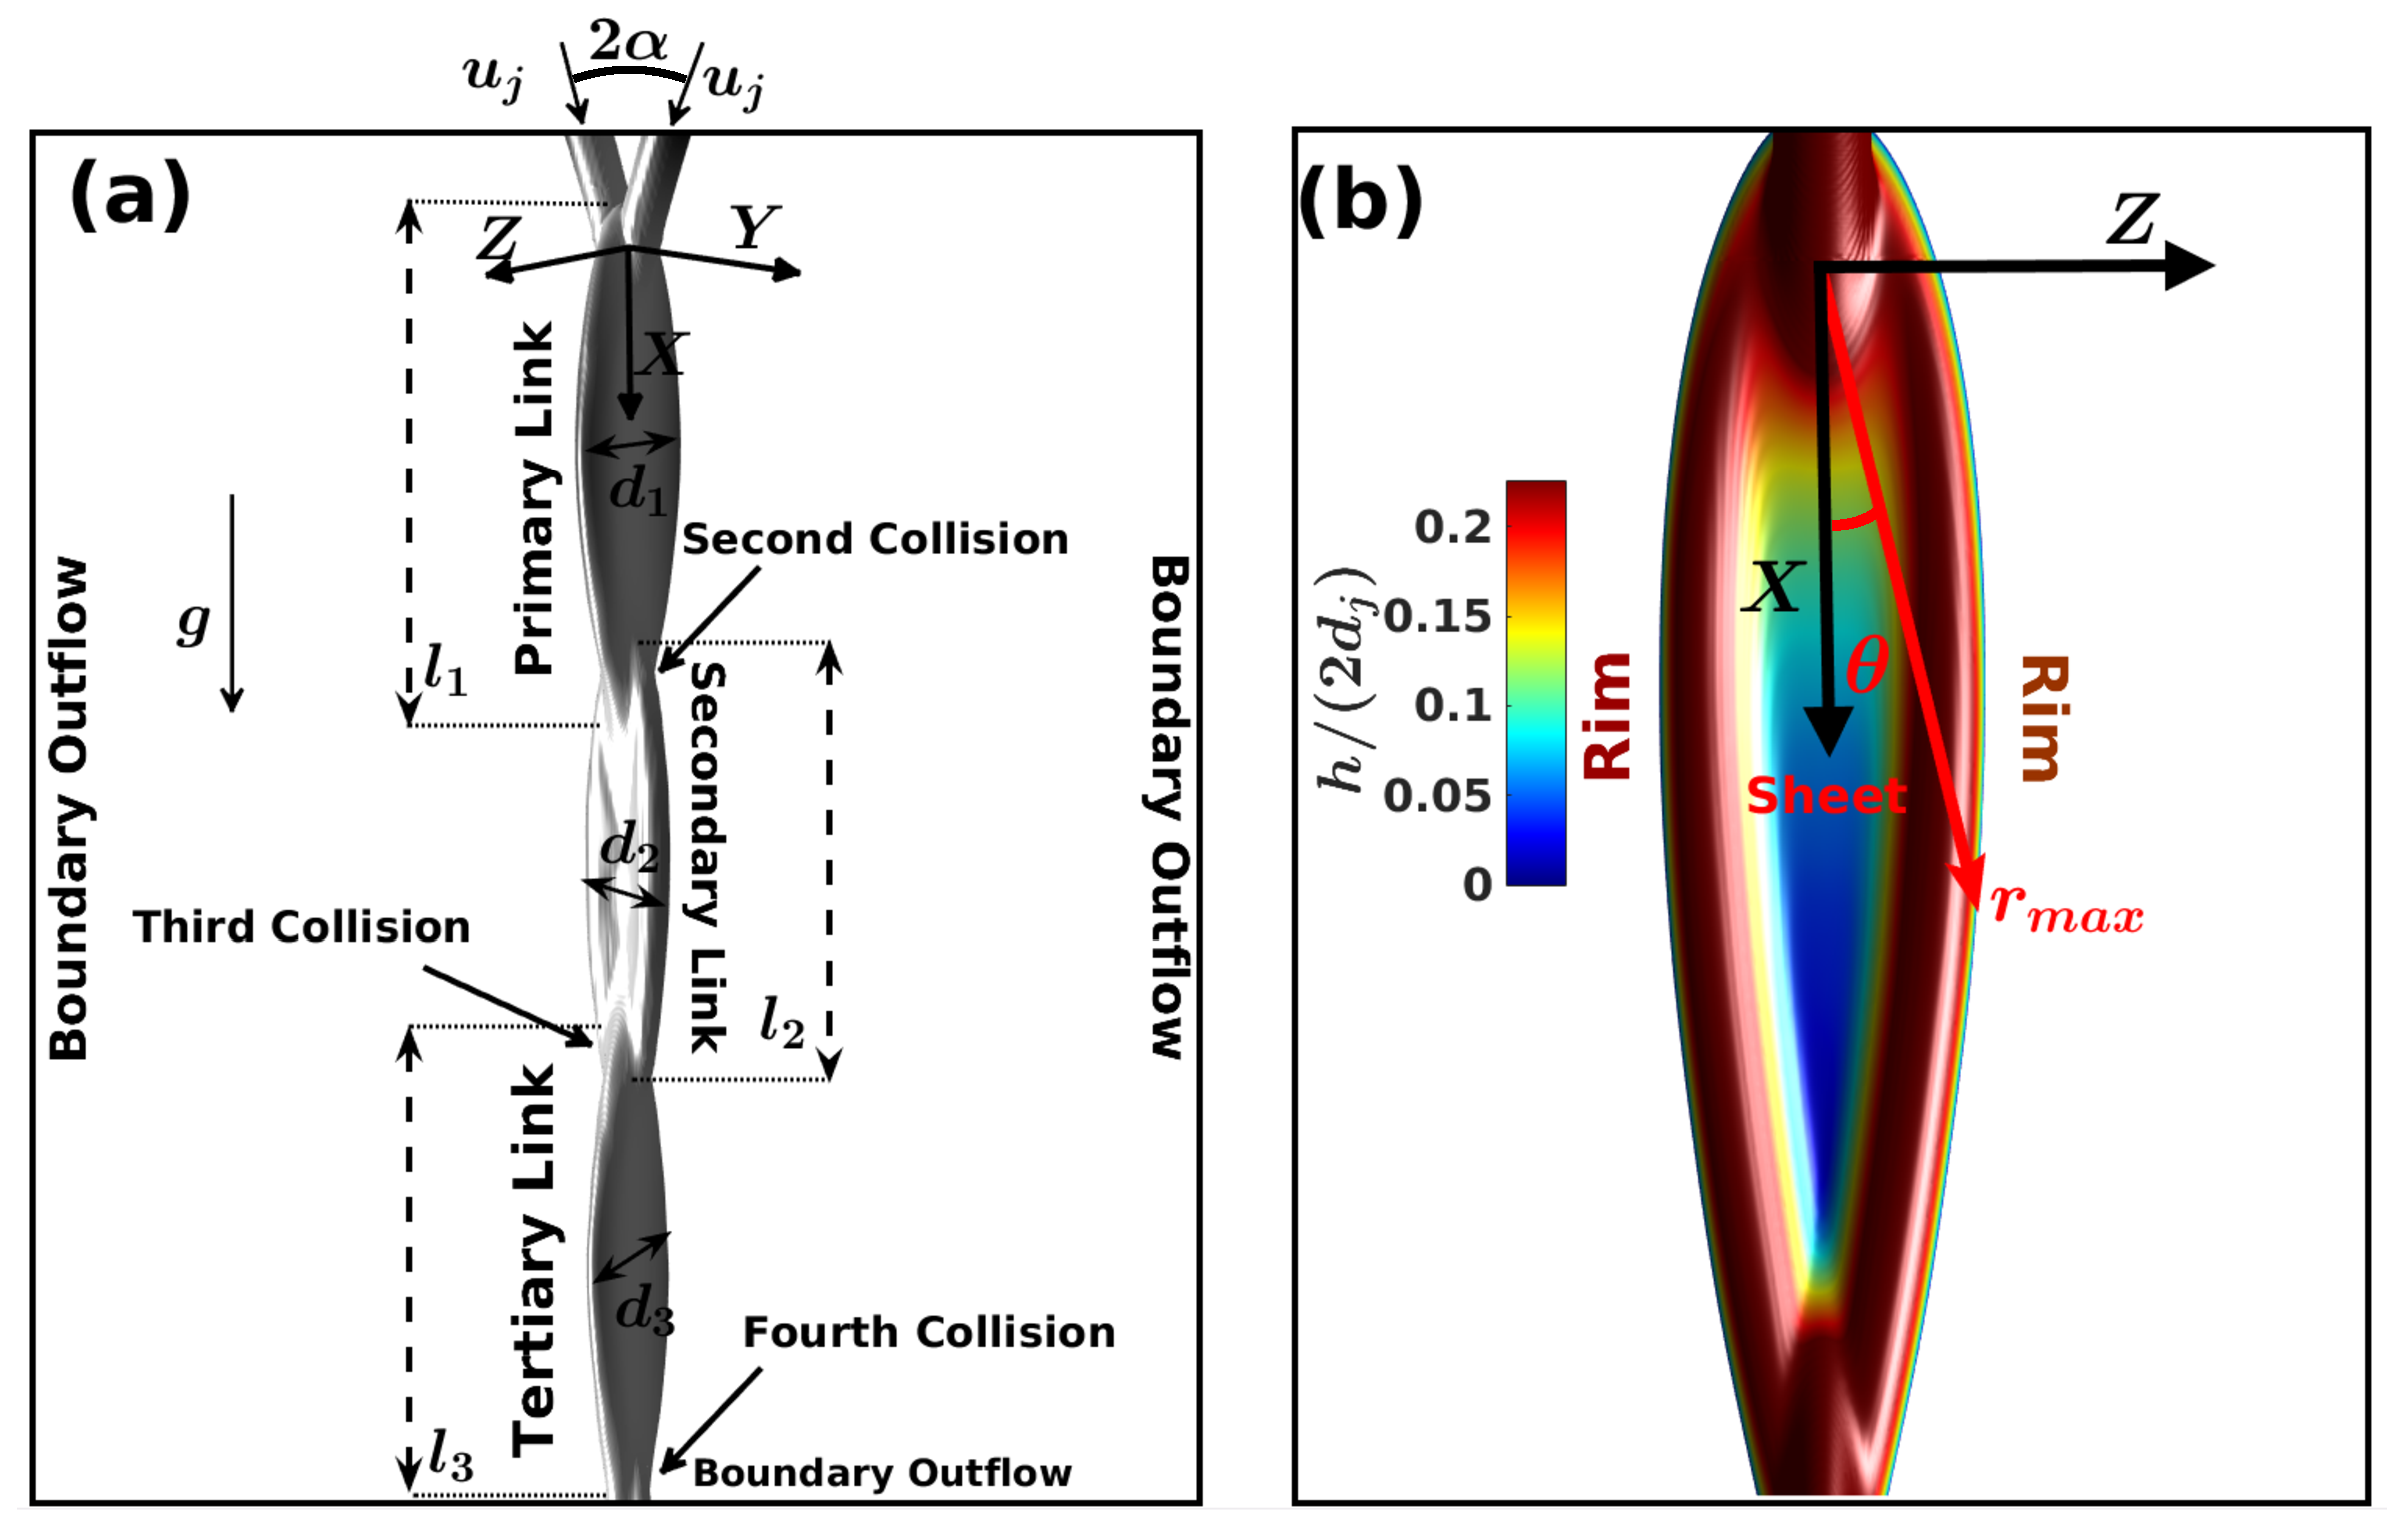
\includegraphics[width=0.75\linewidth]{Figure1}
	\caption{Formation of the liquid sheet by the collision of laminar jets. (a) A schematic to illustrate different structural features and length scales. (b) The primary link structure colored based on half times the magnitude of the sheet thickness, non-dimensionalized with the jet diameter ($\frac{h}{2d_j}$).}
	\label{Figure::schematic}\vspace{-5mm}
\end{figure}
Interactions of liquid jets have invoked the curiosity of researchers with their ubiquitous presence, eminent even in the scientific artworks by Leonardo Da Vinci in the 16$^{th}$ century. Physics of different types of interactions related to liquid jets is classically summarized in a recent effort by \cite{eggers2008physics}. One of these interactions is the collision between liquid jets, presented by \cite{rayleigh1879capillary}. \cite{bush2004collision} introduced several regimes to characterize the different flow structures obtained from such collisions, working on the theory of liquid jet impingement given by \cite{taylor1960formation}. At low velocities or narrow angles of impingement, jets may coalesce to form a unified one or bounce off due to the presence of a thin film of air between them \citep{wadhwa2013noncoalescence}. On increasing the flow rates, laminar jets may lead to the formation of a stable liquid sheet bounded by a thick rim \citep{yang2014liquid}. Inertial and gravitational forces act to expand the liquid sheet formed but the action of surface tension puts a check and allows the sheet to converge, such that the successive collisions of the thick rims downstream of the flow result in the formation of mutually orthogonal liquid sheets \citep{bush2004collision}. Figure~\ref{Figure::schematic}(a) illustrates this structure termed as the liquid chain with the complementary orthogonal sheets forming the different links. Alternatively, further increase in jet velocity, due to several instability modes, leads towards ejection of droplets from the liquid rim \citep{bremond2006atomization}, fluid fishbones \citep{bush2004collision} and flapping sheet \citep{villermaux2002life} associated with atomized drops \citep{ibrahim1991impinging}. The stable chain regime is not just an idealization of the violent flapping, but also holds physical significance for the exploration of fundamental physics behind atomization. Moreover, these structures can be used as wall-free continuous reactors \citep{erni2013free} and are often used as a canonical arrangement for generation of liquid sheets \citep{bush2004collision,taylor1960formation}.\\
Keeping these fascinating applications in mind, a range of experimental works can be found exploring the formation of stable liquid sheets using viscous jets \citep{choo2001parametric,choo2002velocity,bush2004collision}. Using Particle Image Velocimetry (PIV) technique, radial streamlines are observed near the point of impingement and the fluid parcels travel towards the periphery resulting in the formation of the thick rim due to fluid accumulation \citep{choo2002velocity,bush2004collision}. The rim is stable as long as the curvature force developed by surface tension provides the necessary centripetal acceleration as the fluid packets in the rim accelerate owing to loss in gravitational potential \citep{bremond2006atomization}. On balancing the two, \cite{taylor1960formation} developed an expression for the sheet radius which has been found to describe the experimental results of \cite{bush2004collision} reasonably well. Emphasis has been also given by \cite{bush2004collision} for prediction of shapes of leaf-like links forming chain structure. However, the model requires input from the experiments so as to close the system of differential equations. Isolated numerical efforts are also found describing different possible outcomes due to liquid jets interactions. As a part of their study, \cite{chen2013high} have shown the formation of liquid chain using Finite Volume based Volume of Fluid (VOF) network. Recently, \cite{da2016surface} also demonstrated the formation of liquid chain using Boundary Element Method (BEM). But, their exhibition of chain-like structure along with other physical jet related structures suffer from inviscid assumption.\\
Critical assessment of literature reveals that an in-depth study of fluid chain regime is still due which can explore fundamental physics behind the formation of primary link and establish a relation between successive diminishing links. A major challenge that lies in the prediction of the chain-like structure is the proper resolution of the sheet (approximately $1/100^{th}$ of jet diameter) between the rims, which are supposed to mingle once again for forming next link in a mutually perpendicular plane. Figure~\ref{Figure::schematic}(b) is presented to demonstrate the presence of a diversity of length scales in such a simplistic fluid link. In the present work, we attempt the study of an overall behavior of the fluid chain while focusing on the physics of flow for the primary link by analyzing the dimensional characteristics and velocity fields. Special attention is given to the second and third collisions, leading to the formation of the subsequent mutually orthogonal links and relate them from fundamental force balance. In the next section, the numerical framework employed in this work is briefly explained before reporting mesh sensitivity analysis and validation.
\section{Numerical framework}
\begin{figure}
	\centering
	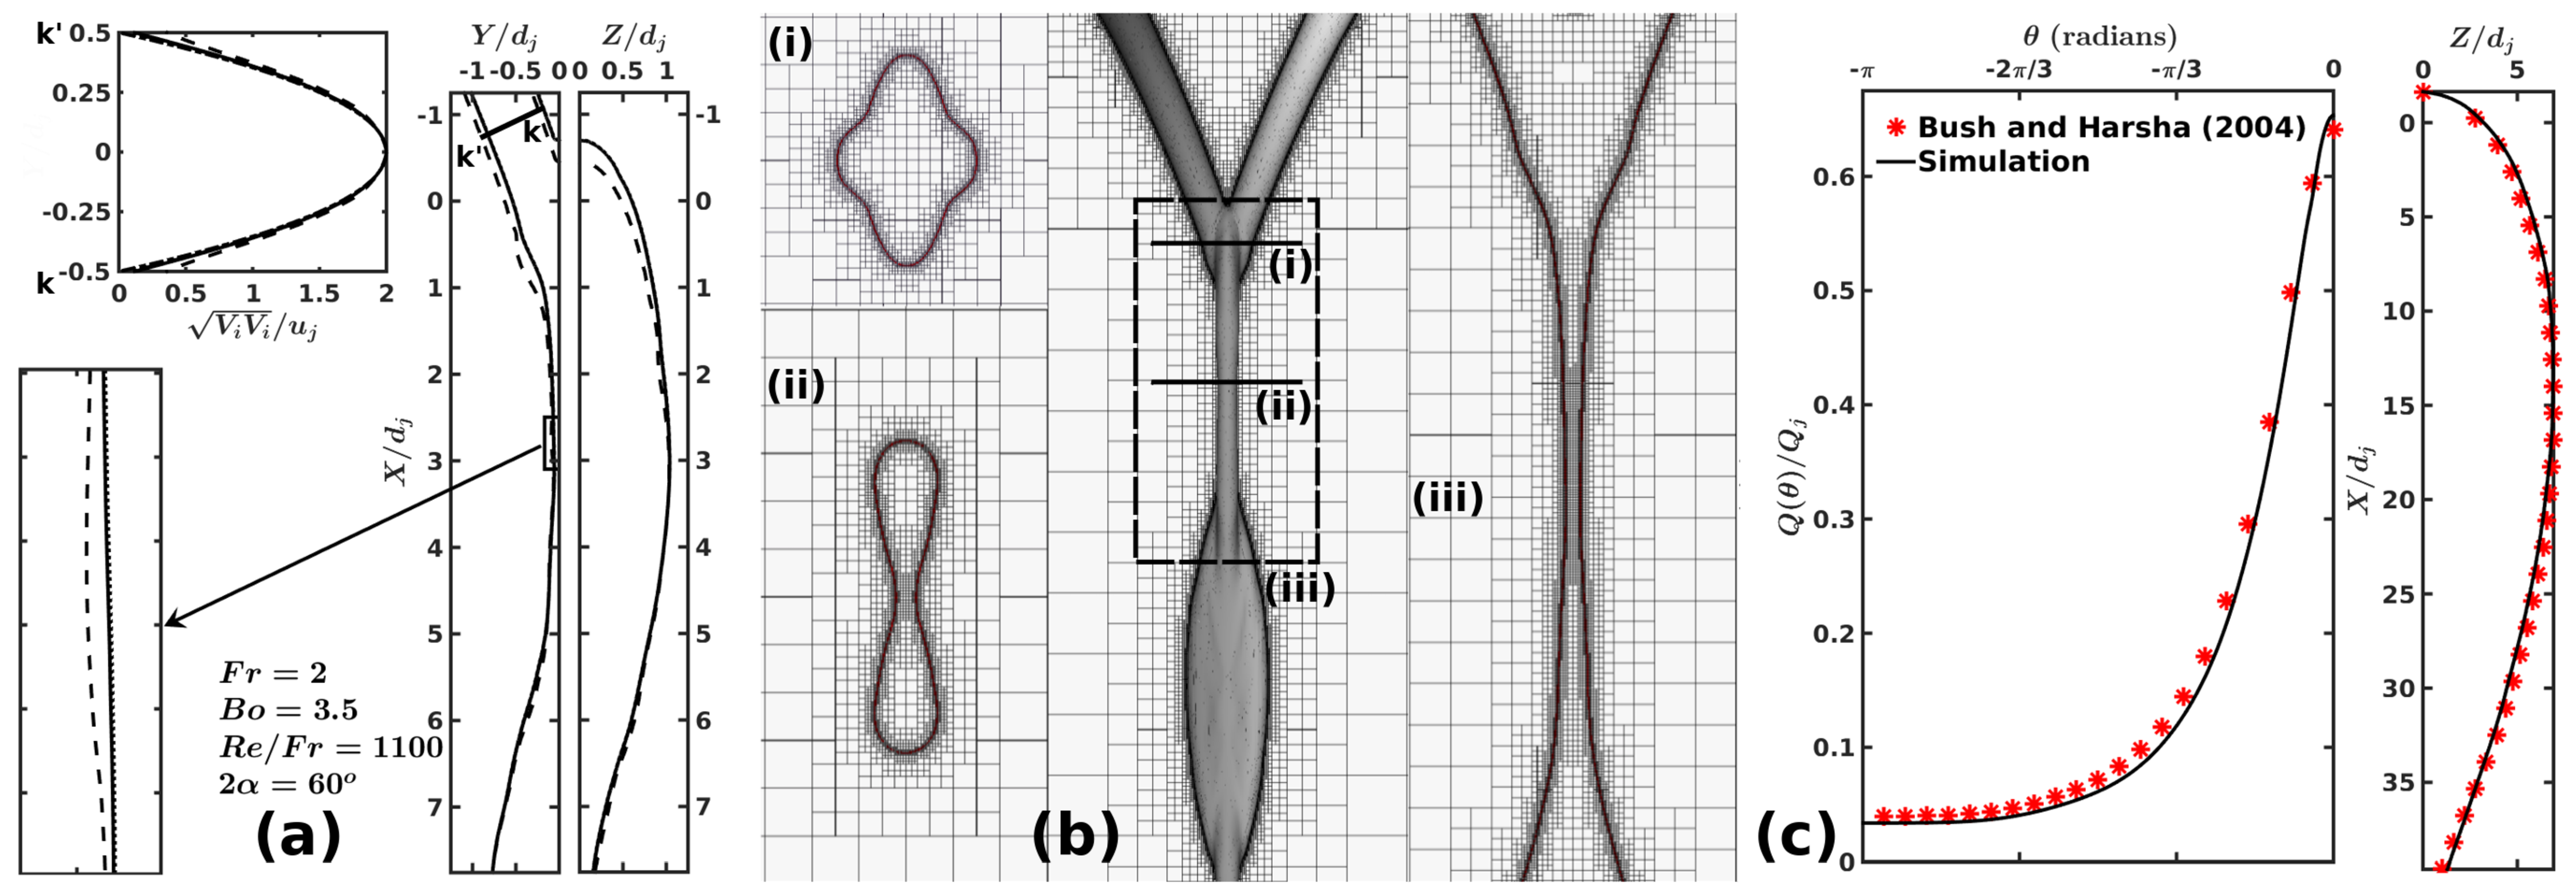
\includegraphics[width=\linewidth]{Figure2}
	\caption{(a) Mesh Sensitivity Analysis for a representative chain structure with outer periphery and velocity profile near the inlet; (b) Representation of the Adaptive Mesh Refinement (AMR) technique at critical locations; (c) Numerical interface (left) and Liquid flux (right) superimposed with the respective experimental values obtained by \cite{bush2004collision} to depict validation.}
	\label{Figure::gisetal}
\end{figure}
The collision of liquid jets has been studied in three-dimensional finite volume framework. Open source, time-dependent, multi-fluid, Navier-Stokes solver, Gerris is used for the current study \citep{Popinet2003}. The spatial discretization of the domain is undertaken using an octree based structured hierarchical grid system, locally refined near the interface. Conventional mass and momentum conservation equations for incompressible flow have been solved in presence of interface specific surface tension force ($\sigma \kappa$, where $\sigma$ is the surface tension coefficient and $\kappa$ denotes the curvature of the interface) and gravitational field ($\rho g$). The interface tracking is undertaken using the Volume Of Fluid (VOF) approach using volume fraction of liquid, defined as $\Psi(x_i, t)$, at the spatial and temporal instance of $x_i$ and $t$ respectively. Therefore, the density and viscosity for the study can be described using equation~\ref{Equation::general}.
\begin{equation} \label{Equation::general}
A (\Psi) = \Psi A_1 + (1-\Psi)A_2 \: \: \:  \forall  \: A \in \{\rho, \mu\}
\end{equation}
The VOF approach is implemented in a two-step process of interface reconstruction (based on the values of $\Psi$ and piecewise linear interface construction scheme, PLIC) along with geometric flux computation and interface advection, shown in equation~\ref{Equation::vof}.
\begin{equation} \label{Equation::vof}
\frac{\partial \Psi}{\partial t} + \frac{\partial(\Psi V_i)}{\partial X_i} = 0
\end{equation}
Gerris uses second order accurate time discretization of momentum and continuity equations with time splitting algorithm as proposed by \cite{Chorin1968}, whereby an unconditionally stable corrector predictor time marching approach is adopted. A multi-grid solver is used for the solution of the resulting pressure-velocity coupled Laplace equation. The advection term of the momentum equation $\left(V_k\frac{\partial V_i}{\partial X_k}\right)$ is estimated using the Bell-Colella-Glaz second-order unsplit upwind scheme \citep{bell1989second}, which requires the restriction to be set up on the time step. Following \cite{popinet2009}, time step has been determined to satisfy Courant-Friedrich-Lewy (CFL) stability criteria of less than unity. The details of solution procedure can be found in the works of \cite{Popinet2003,popinet2009}.\\
The computational domain is also illustrated in figure~\ref{Figure::schematic}(a) with parabolic inflow (average velocity, $u_j$) of jets (diameter, $d_j$ and impingement angle, $2\alpha$) and boundary outflow elsewhere. From the works of \cite{choo2001parametric}, it can be easily shown that the thickness of liquid sheet follows $\frac{hr}{d_j^2} \sim 1$, for $2\alpha \in \{0,\pi/2\}$.  Here, $r$ is the radial direction originating from the collision point of the jets and h is the measurement of the thickness of the film produced when jets collide. We maintained $\frac{d_j}{\delta l} \sim 10\frac{r_{max}}{d_j}$ to choose minimum cell size $\left(\delta l\right)$ and perform Grid Independence Study (GIS). The factor of 10 is included to have at least 10 grid points\citep{ling2015multiscale} across the smallest length scale for the structure to avoid breakage of sheet \citep{chen2013high}. To obtain continuous liquid film and well-resolved phenomenon, $\delta l$ is varied to match the above-mentioned criteria. In one representative simulation, we show the effect of variation of $\delta l$, in figure~\ref{Figure::gisetal}(a), on sheet profile and velocity pattern of the jet. It can be observed that at $\frac{d_j}{\delta l}$ = 102.4, well resolved film is obtained with acceptable computational cost ($\sim 50\%$ less than $\frac{d_j}{\delta l}$ = 204.8). Mesh structure around different critical parts of the chain is shown in figure~\ref{Figure::gisetal}(b) which establishes sufficiency of grid points even inside smallest thickness of the film. To check the accuracy of the developed mesh structure, results from simulations are compared (figure~\ref{Figure::gisetal}(c)) with experimental observations of sheet profile reported by \cite{bush2004collision}. So as to get quantitative validation, the variation of liquid volume flux inside the sheet is also plotted in figure~\ref{Figure::gisetal} along with \cite{bush2004collision}. In both the cases, matching between present numerical simulations and pioneering experimental result by \cite{bush2004collision} provides confidence for the numerical understanding of the phenomenon, in our work. Further, on performing non-dimensional analysis, it can be observed that Froude number $\left(Fr = \frac{u_j}{\sqrt{gd_j}}\right)$, Bond number $\left(Bo = \frac{\rho gd_j^2}{\sigma}\right)$ and ratio between Reynolds number and jet Froude number $\left(Re/Fr = \frac{\rho\sqrt{gd_j^3}}{\mu}\right)$ govern the shape and sizes of different links in the fluid chain structure. In our next section, a detailed effort has been presented to investigate the formation of the chain based on above non-dimensional numbers.
\section{Collision and Sheet Formation}
\begin{figure}
	\centering
	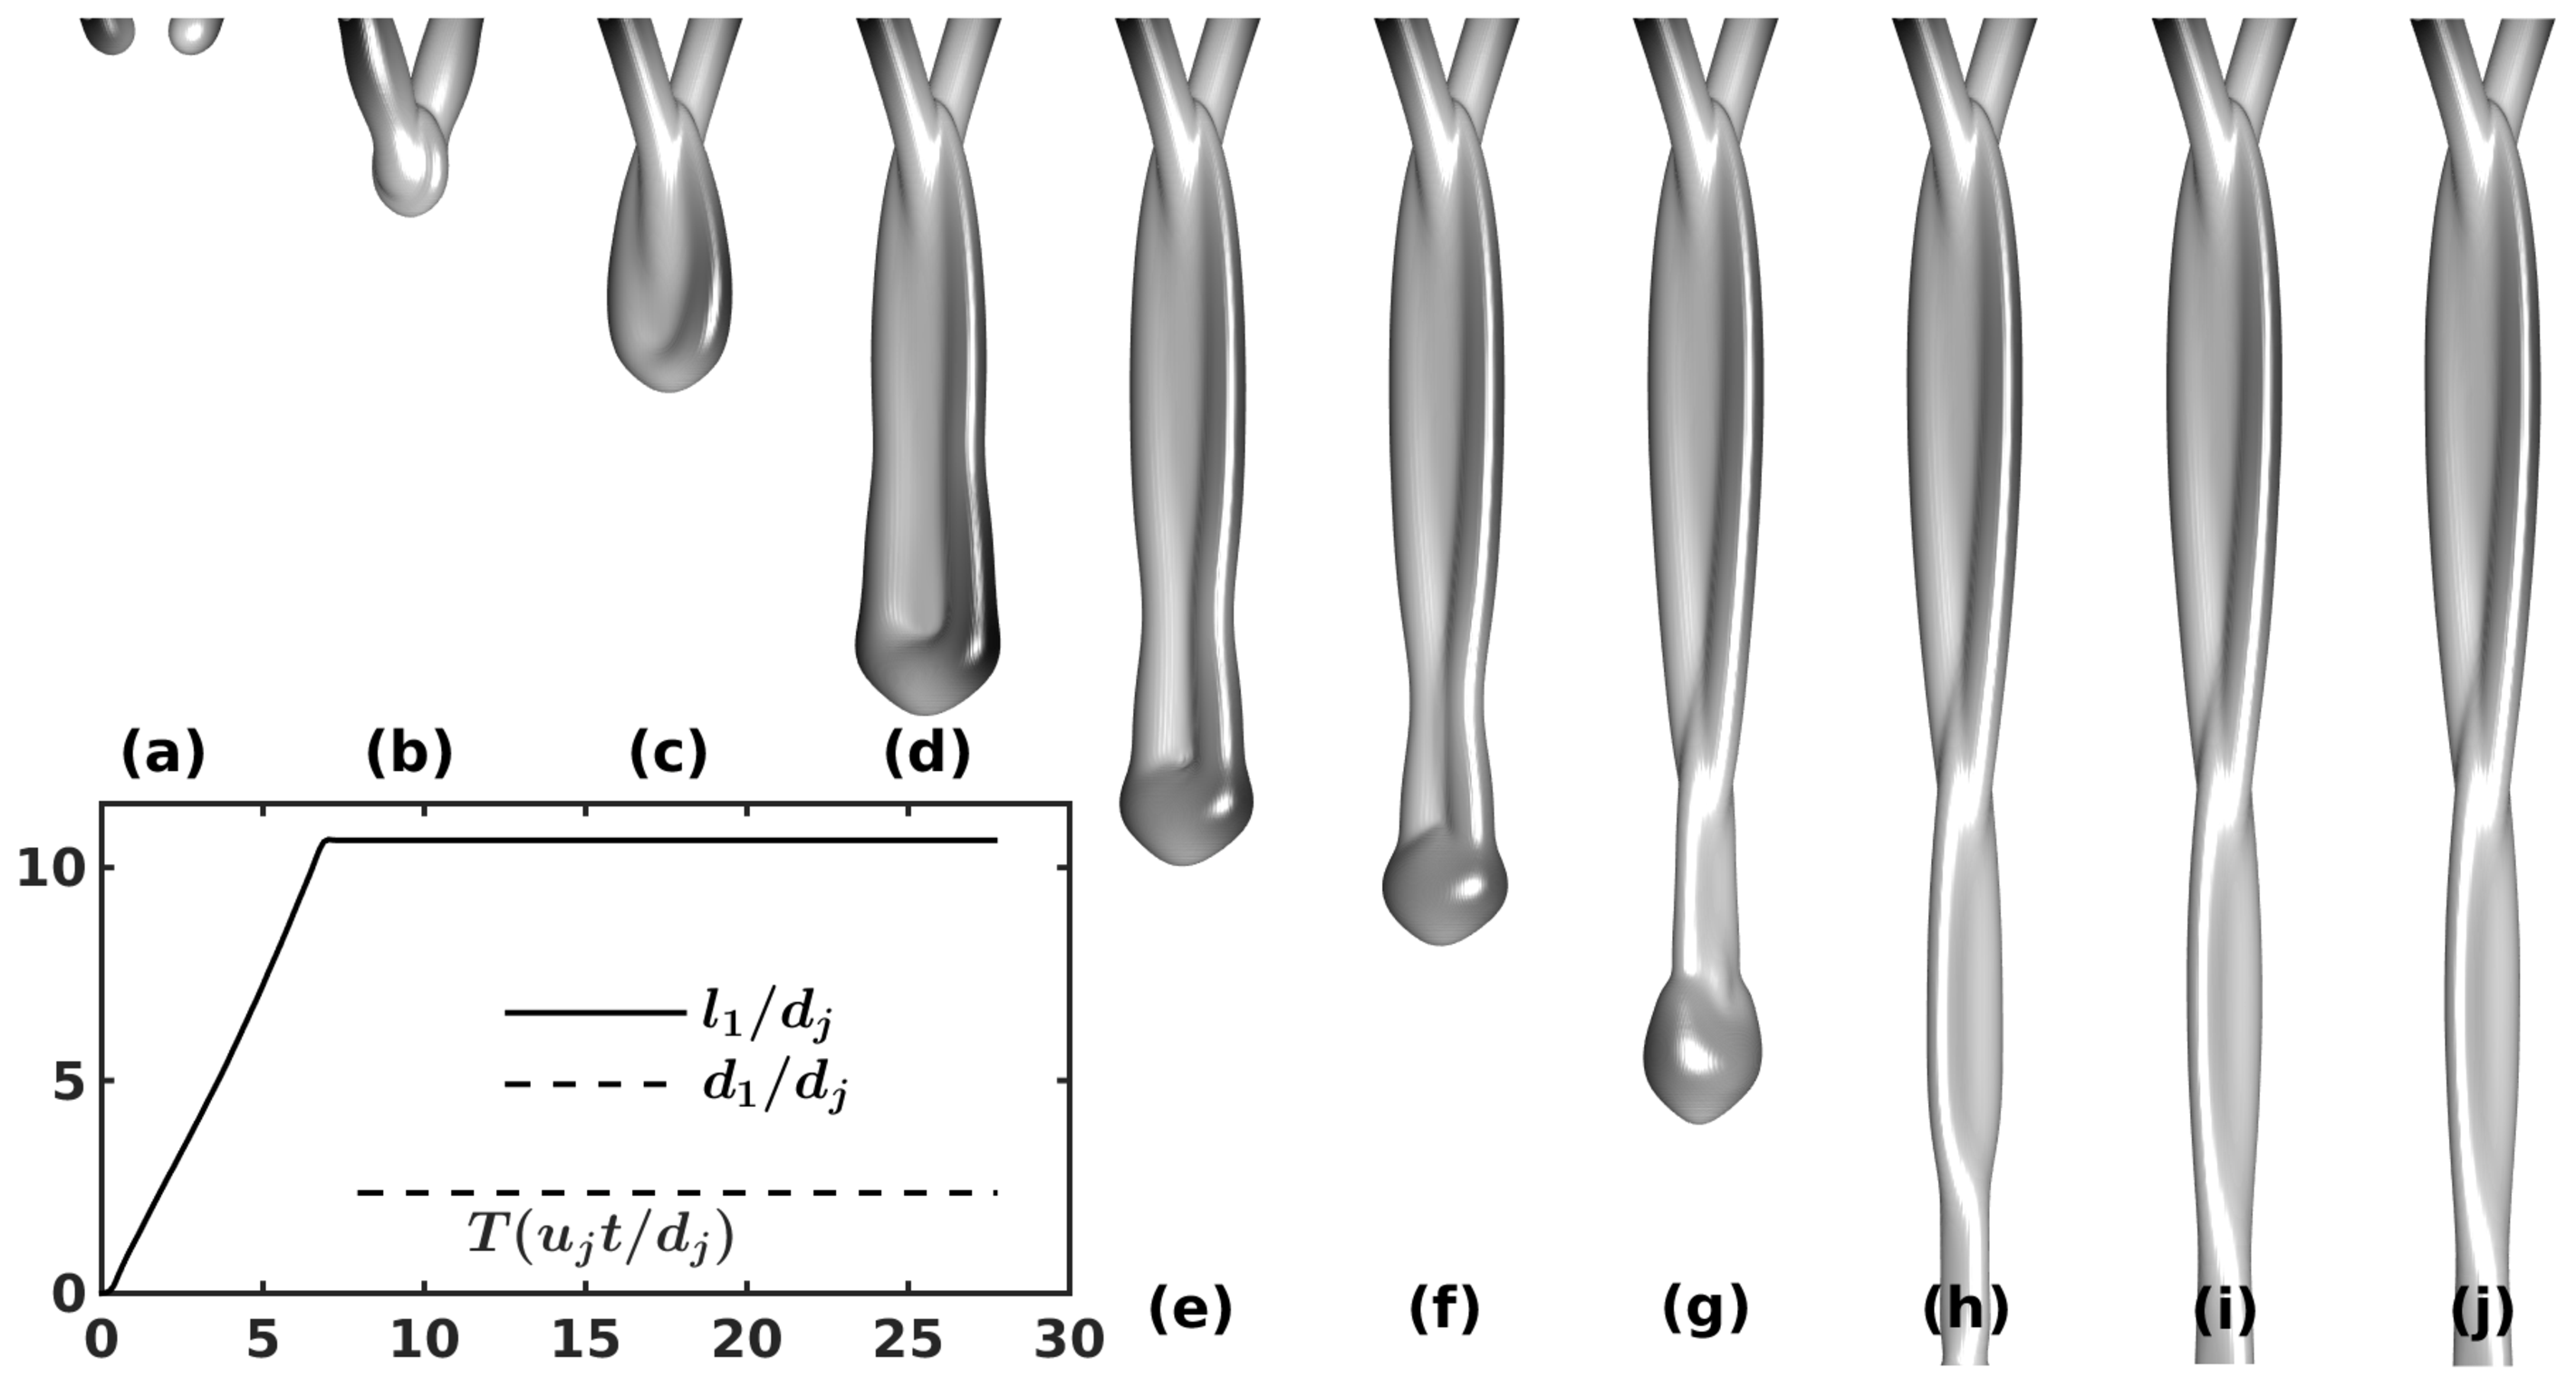
\includegraphics[width=0.6\linewidth]{Figure3}
	\caption{Transition to the steady state fluid-links chain formed by collision of laminar jets. The figure illustrates the transient period through the temporal advancement from (a) pre-collision symmetric jets to $T (\frac{u_jt}{d_j}) = $ (b) 1.5, (c) 4, (d) 5, (e) 5.5, (f) 6.5, (g) 8.5, (h) 16.5, (i) and (j) 20}
	\label{Figure::transient}\vspace{-3.2mm}
\end{figure}
As the laminar liquid jets collide, a thin sheet bounded by thicker rims is formed in the median plane, perpendicular to the axes of the jets. In this section, the formation process of chain structure due to the collision of liquid jets is discussed. Figure~\ref{Figure::transient} shows temporal evolution of the fluid sheet when the two jets collide. The fluid parcels are dispatched radially outwards from the point of impingement. This along with net inertia of jets and gravity results in a bay leaf like sheet as shown in figures~\ref{Figure::transient}(b) and~\ref{Figure::transient}(c). Present zone of consideration lies in 0.5 $< Fr <$ 4, where gravity plays a major role unlike \cite{bush2004collision,bremond2006atomization}.
In absence of surface tension or at very high Weber number, the sheet will keep on expanding (figures~\ref{Figure::transient}(d) and~\ref{Figure::transient}(e)), leading to the formation of the open rim structures \citep{taylor1960formation,chen2013high}. As the sheet closes onto itself, the two rims at the periphery undergo a second oblique collision (figure~\ref{Figure::transient}(f)) at an angle smaller than the initial collision (figure~\ref{Figure::transient}(b)). After the secondary impingement, similar to figure~\ref{Figure::transient}(c), a flow biased sheet begins to develop (figure~\ref{Figure::transient}(g)). Formation of this secondary link has no effect on the characteristics features of the primary link as the sheet speed is supercritical \citep{bush2004collision}, and therefore can be independently studied. Temporal advancement results in the formation of a full-fledged secondary link as shown in figure~\ref{Figure::transient}(h). It must be noted that the plane of formation of this sheet is orthogonal to that of the primary link and therefore the secondary link shares the same plane as the axes of the jets. The process continues and a series of mutually orthogonal links are obtained, successively reducing in size until a long single liquid jet is formed \citep{bush2004collision}. After the initial transients, links become steady $\left(T\right. \left(\frac{u_jt}{d_j}\right) $ = 8.5 as representation in primary link$\left.\right)$ which has been analyzed further. \\
Jets progress towards each other and collide at a point in the median sheet plane to form a sheet bounded by leaf-like rims. Fast moving, the thin sheet possess radial velocity pattern emerging from a stagnation point, $\delta s$ higher than the impingement location. \cite{inamura2014effect} have established $\delta s = \lambda d_j/(2\sin\alpha)$, where the factor $\lambda$ is a function of the impingement angle. Considering $\delta s$ and velocity vectors obtained from numerical simulations for two sets of non-dimensional numbers, flow pattern inside the sheet is reported in figure~\ref{Figure::velocityVectors}(a). It can be observed that velocity vectors follow a self-similar smooth path, as traced by sheet boundary. An increase of sheet span can be also noticed from the figure for an improved velocity of impacting jets.  
An effort has been made to observe the steady average flow $\left(u_f(r,\theta)\right)$ across the thickness of the sheet at a given radial and azimuthal point. It can be expressed as equation~\ref{Equation::uf}. 
%$u_f(r,\theta) = \int_{0}^{1}\sqrt{V_iV_i}d(Y/h)$. 
\begin{equation}\label{Equation::uf}
u_f(r,\theta) = \int_{0}^{1}\sqrt{V_iV_i}d(Y/h)
\end{equation}
Variation of $u_f(r,\theta)$ along radial plane at different azimuthal angles have been shown in figure~\ref{Figure::velocityVectors}(b). It can be observed that the order of change in the fluid velocity across the radial distance from the point of impact is less than the change across the azimuthal direction \citep{choo2002velocity}. Further, sheet velocity $\left(u_s(\theta)\right)$ along a radial plane has been also obtained by integrating $u_f(r,\theta)$ as: %$u_s(\theta) = \int_{0}^{1}u_f(r,\theta)d(r/r_{max})$.
\begin{equation}\label{Equation::us}
u_s(\theta) = \int_{0}^{1}u_f(r,\theta)d(r/r_{max})
\end{equation} 
Upon non-dimensionalization of sheet velocity with its average $\left(u_0\right)$, a self-similar behavior in azimuthal direction is observed for a wide diversity of non-dimensional parameters reported in figure~\ref{Figure::velocityVectors}(c). In this figure, four arbitrarily chosen parameters are shown which adheres to a function relationship of $u_s(\theta)$ in the following fashion: 
\begin{equation}\label{Equation::usu0}
\frac{u_s(\theta)}{u_0} = 1.03 + 0.13\cos\left(\frac{4.18\theta}{\pi}\right)
\end{equation}
Once the average sheet velocity exceeds a critical value, the chain structure is no longer stable as the  Kelvin - Helmholtz instability kicks in \citep{villermaux2002life}. \\
\begin{figure}
	\centering
	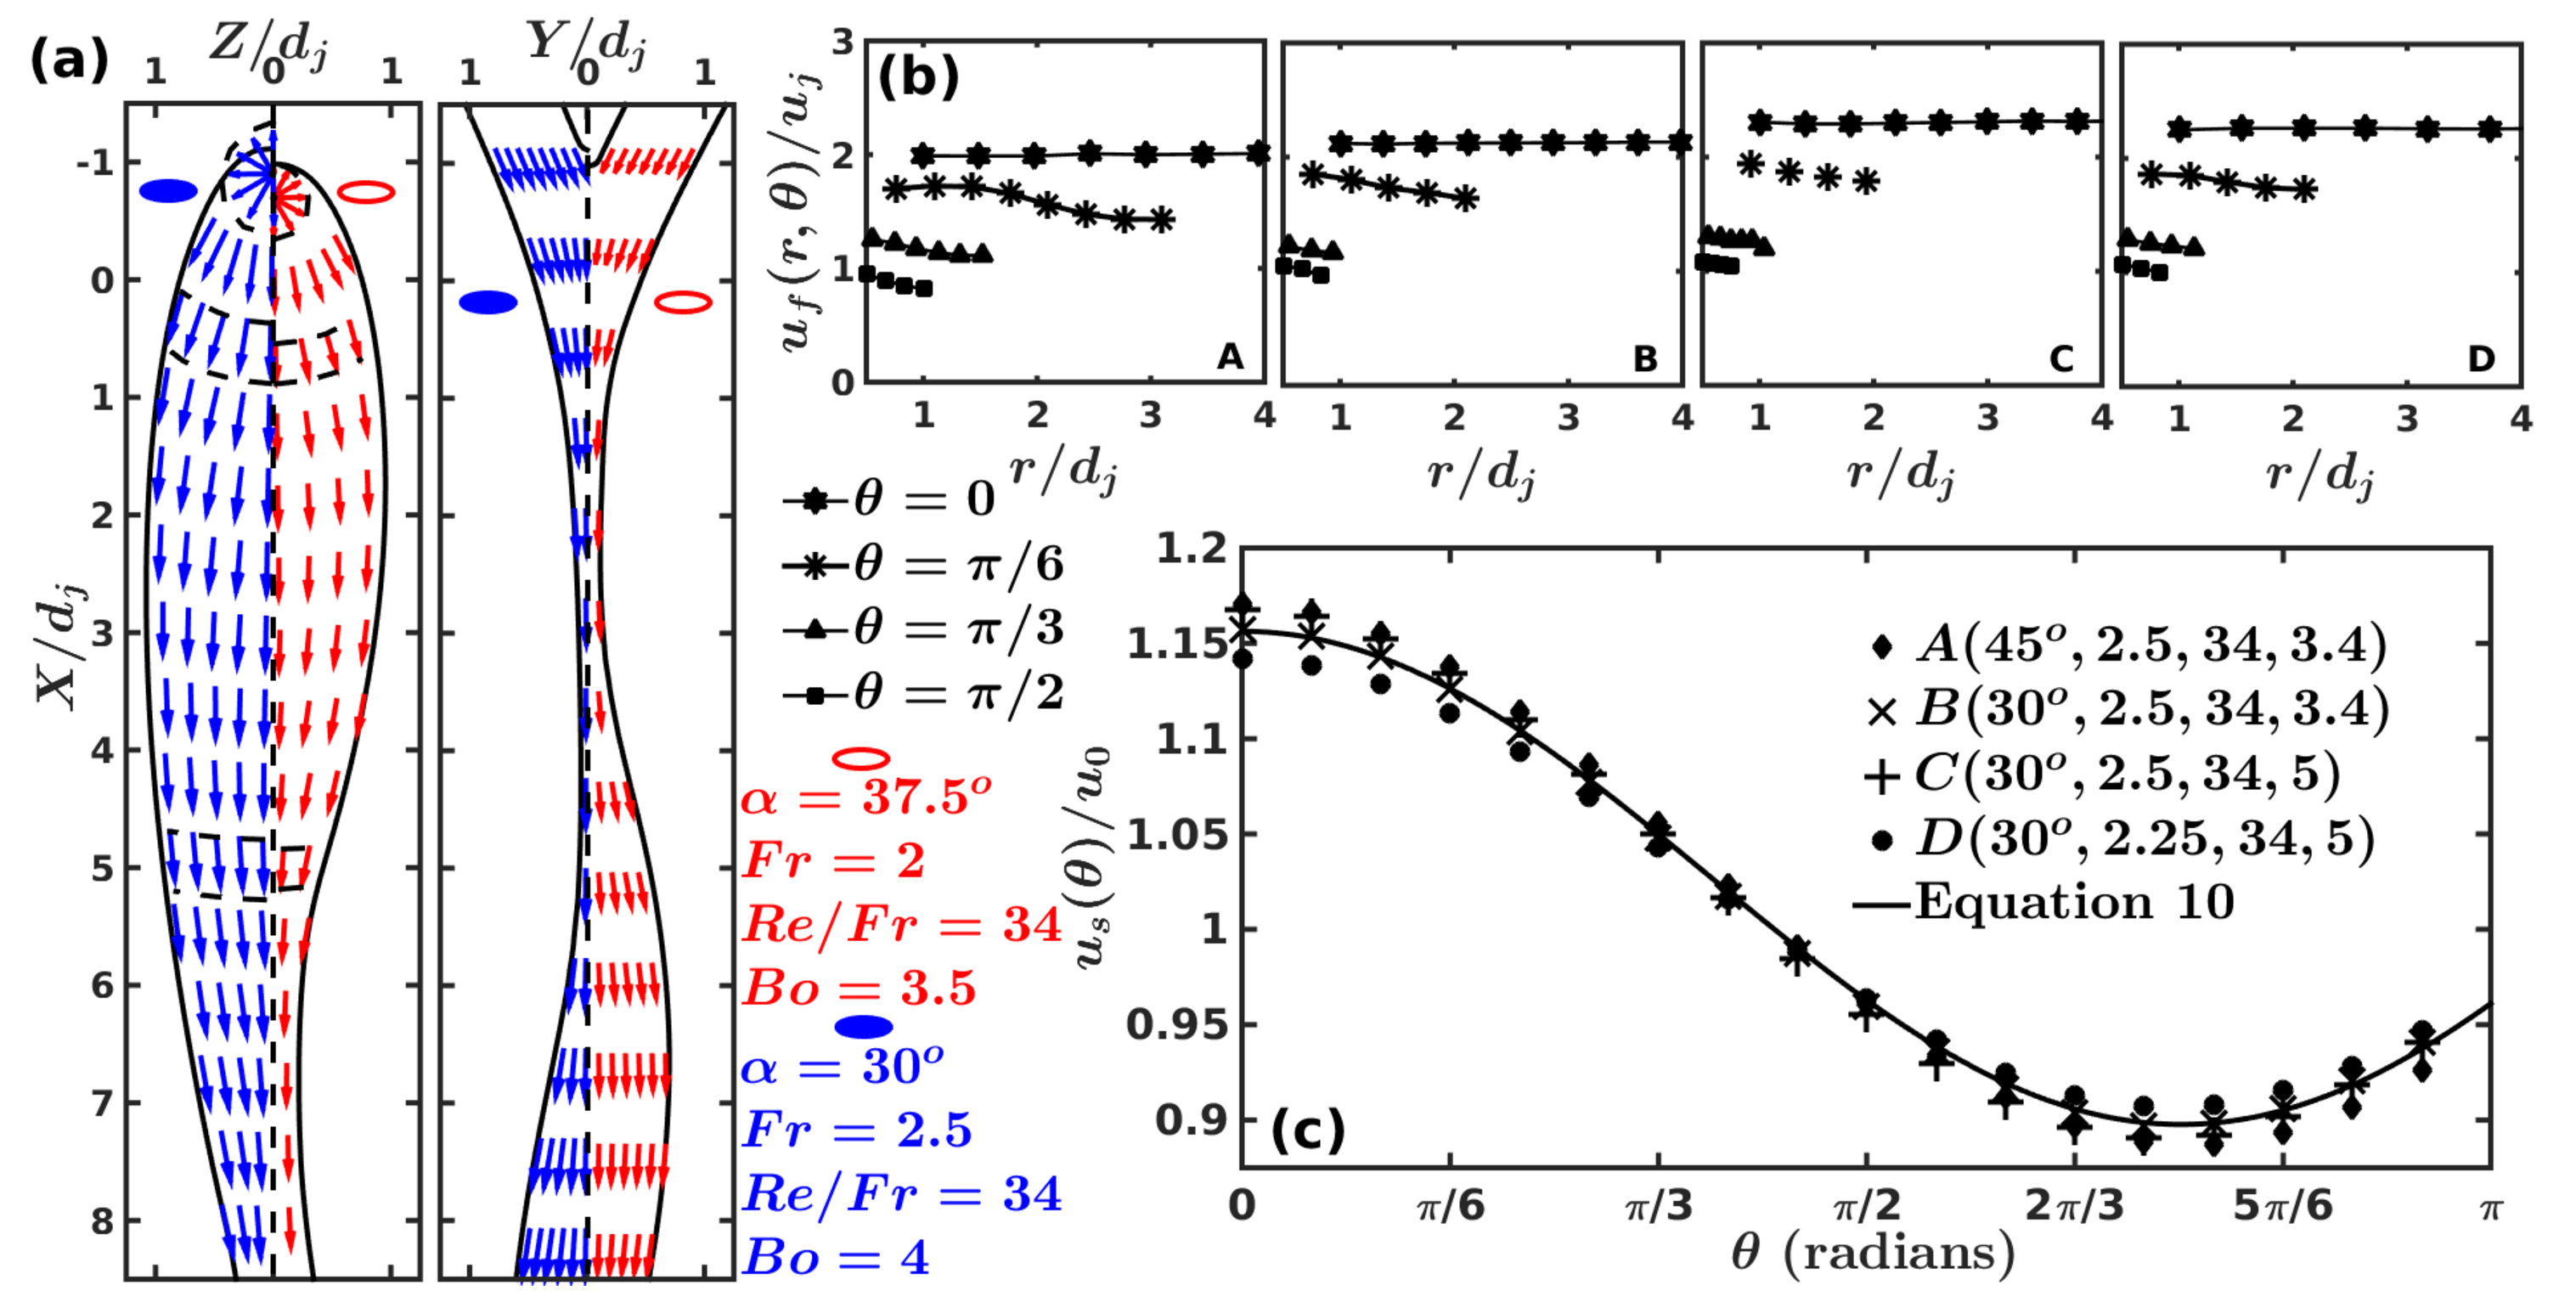
\includegraphics[width=\linewidth]{Figure4}
	\caption{Flow kinematics of the fluid parcels: (a) Velocity vector field for two representative cases, (b) Variation of velocity in the radial direction for four representative cases and (c) Variation of the radially averaged sheet velocity $\left(u_s(\theta)\right)$, non-dimensionalized with the average sheet velocity $\left(u_0\right)$ along the azimuthal direction in the sheet.}
	%\caption{Flow kinematics of the fluid parcels: (a) Velocity vector field for two representative cases; the vector field is radial near the stagnation point and then follows the self similar phase contour, (b) Variation of velocity in the radial direction for four representative cases with ($\alpha$, $Fr$, $Re/Fr$, $Bo$): A(45$\degree$, 2.5, 34, 3.4), B(30$\degree$, 2.5, 34, 3.4), C(30$\degree$, 2.5, 34, 5) and D(30$\degree$, 2.25, 34, 5) and (c) Variation of the radially averaged sheet velocity ($u_s$), non-dimensionalized with the average sheet velocity ($u_0$) along the azimuthal direction in the sheet.}
	\label{Figure::velocityVectors}%\vspace{-2.75mm}
\end{figure}
\begin{figure}
	\centering
	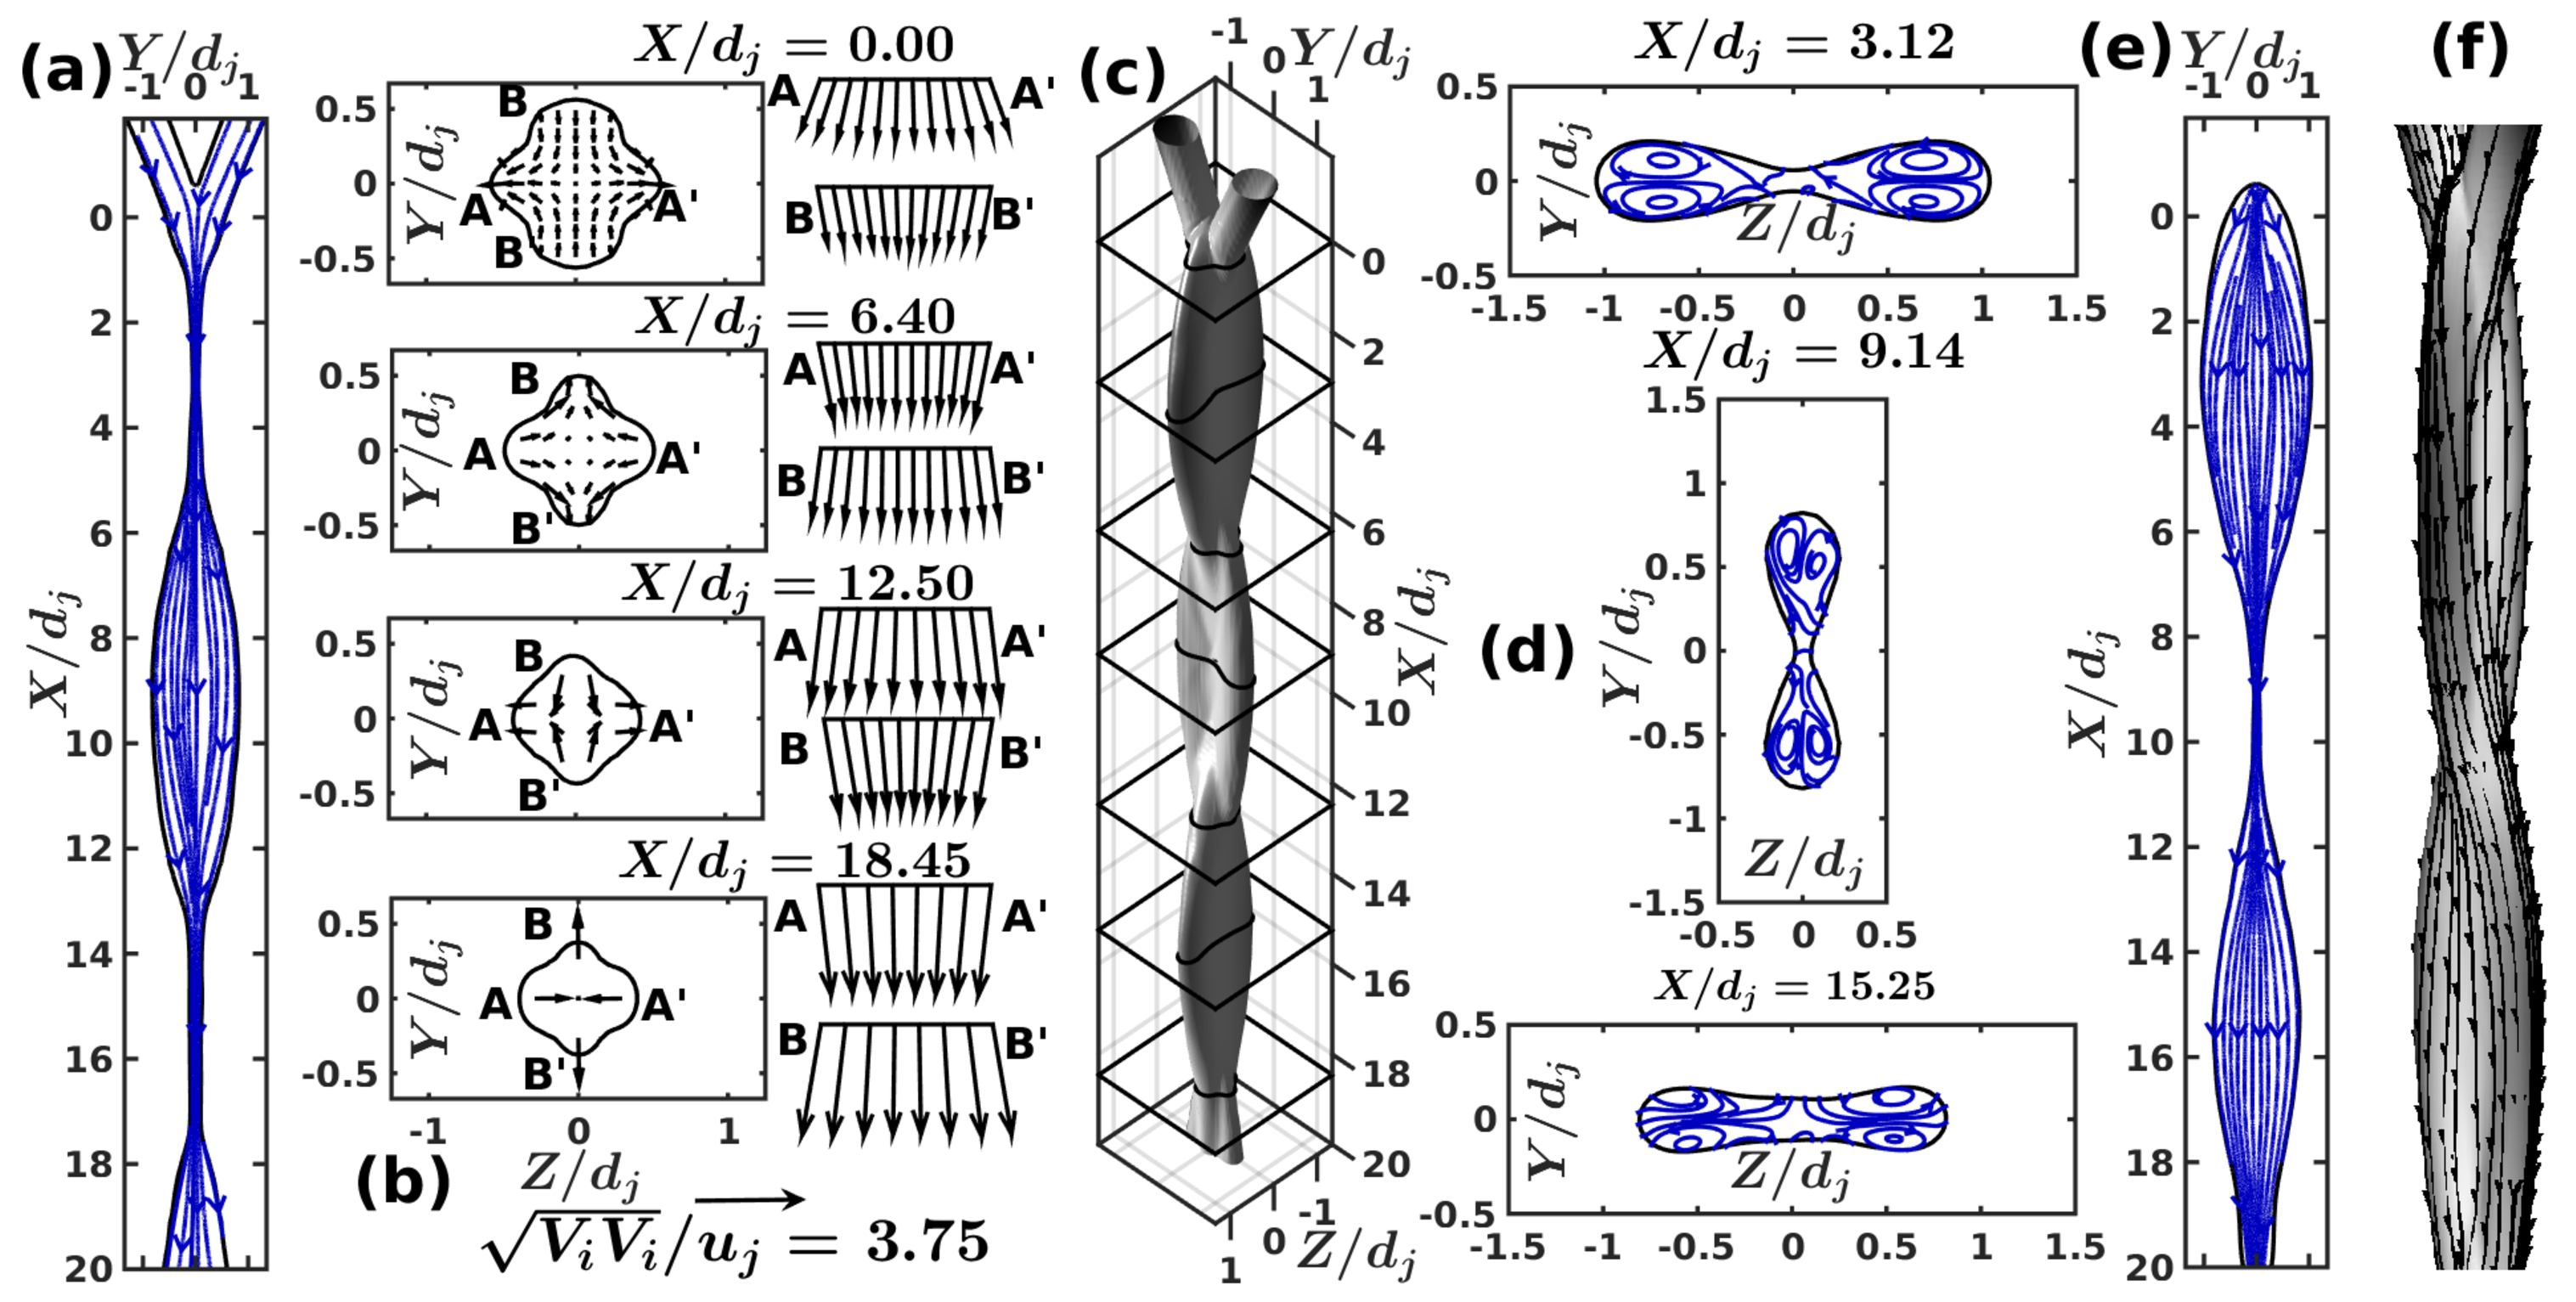
\includegraphics[width=\linewidth]{Figure5}
	\caption{Three dimensional velocity field for $\alpha$ = 30$\degree$, $Fr$ = 2,  $Re/Fr$ = 1125 and $Bo$ = 3.4 with (a) XY plane streamlines, (b) Velocity vector field in the YZ plane at different collision locations, (c) The three dimensional stable chain structure, (d) Streamlines at maximum link widths in the YZ plane, (e) XZ plane streamlines and for $\alpha$ = 30$\degree$, $Fr$ = 2,  $Re/Fr$ = 1725 and $Bo$ = 3.4 with (f) Three dimensional streamlines embedded onto the chain structure.}
	\label{Figure::streamDetails}%\vspace{-2.75mm}
\end{figure}
An overall look of three-dimensional chain structure (figure~\ref{Figure::streamDetails}(c)) allows us to obtain velocity patterns at different axial locations. The streamlines follow steadily the phase contour boundary, with those inside the chain structure going in trajectories similar to the outer boundary as shown in figures~\ref{Figure::streamDetails}(a) and~\ref{Figure::streamDetails}(e). Figure~\ref{Figure::streamDetails}(b) puts an effort towards highlighting velocity vectors at primary, secondary and tertiary links. One can observe from figure~\ref{Figure::streamDetails}(b) that the spread of liquid influence at collision planes is reducing continuously as $X/d_j$ increases.  At $X/d_j$ = 0, the liquid jets converge onto themselves (B-B') marked by retracting velocity field, whereas the liquid sheet grows (A-A') in the Z direction, marked by an expanding velocity field. Similar trends are observed at all collision planes ($X/d_j$ = 6.4, 12.5 and 18.45) leading to the formation of three visible links in this case (figure~\ref{Figure::streamDetails}(c)). The velocity vector magnitudes go on increasing at each subsequent collision planes as the gravitational head is converted to dynamic head leading to narrowing of the extent of liquid phase boundary in the XZ plane. In the primary link, this converging-diverging trend is continued from above the first collision point to the plane where the extent of the link perpendicular to the net flow direction in the plane of the link is maximum. As illustrated in figure~\ref{Figure::streamDetails}(d), the streamlines at the location of maximum width imply that the component of velocity perpendicular to the liquid sheet phase boundary is zero ($\frac{d\Psi}{dn}$ = 0). This results in the formation of distinguished circulation patterns inside the lobes at the locations of the maximum extent corresponding to the three links visible in this case. Reduction of collision strength at different planes explains diminishing spans of the links, which can be also seen from sheet cross-sectional images (figure~\ref{Figure::streamDetails}(d)). A characteristic twist can be found in streamlines (figure~\ref{Figure::streamDetails}(f)) as the flow propagates downstream through the locations of subsequent collisions. The twist occurs as the fluid parcels are restricted by surface tension to follow the chain outer periphery. These twists are prominent until viscous effects take charge and only a single jet of liquid is left at the end of the chain structure. These viscous forces lead to dissipation of energy as the liquids jets (or rims for the post-primary link) collide with each other. It is clear from our discussions above that, different flow parameters, characterized by non-dimensional numbers play a crucial role in the determination of the three-dimensional stable chain structures and therefore, the next section is devoted to analyzing such effects.
\section{Assessment of factors influencing chain structure}
\begin{figure}
	\centering
	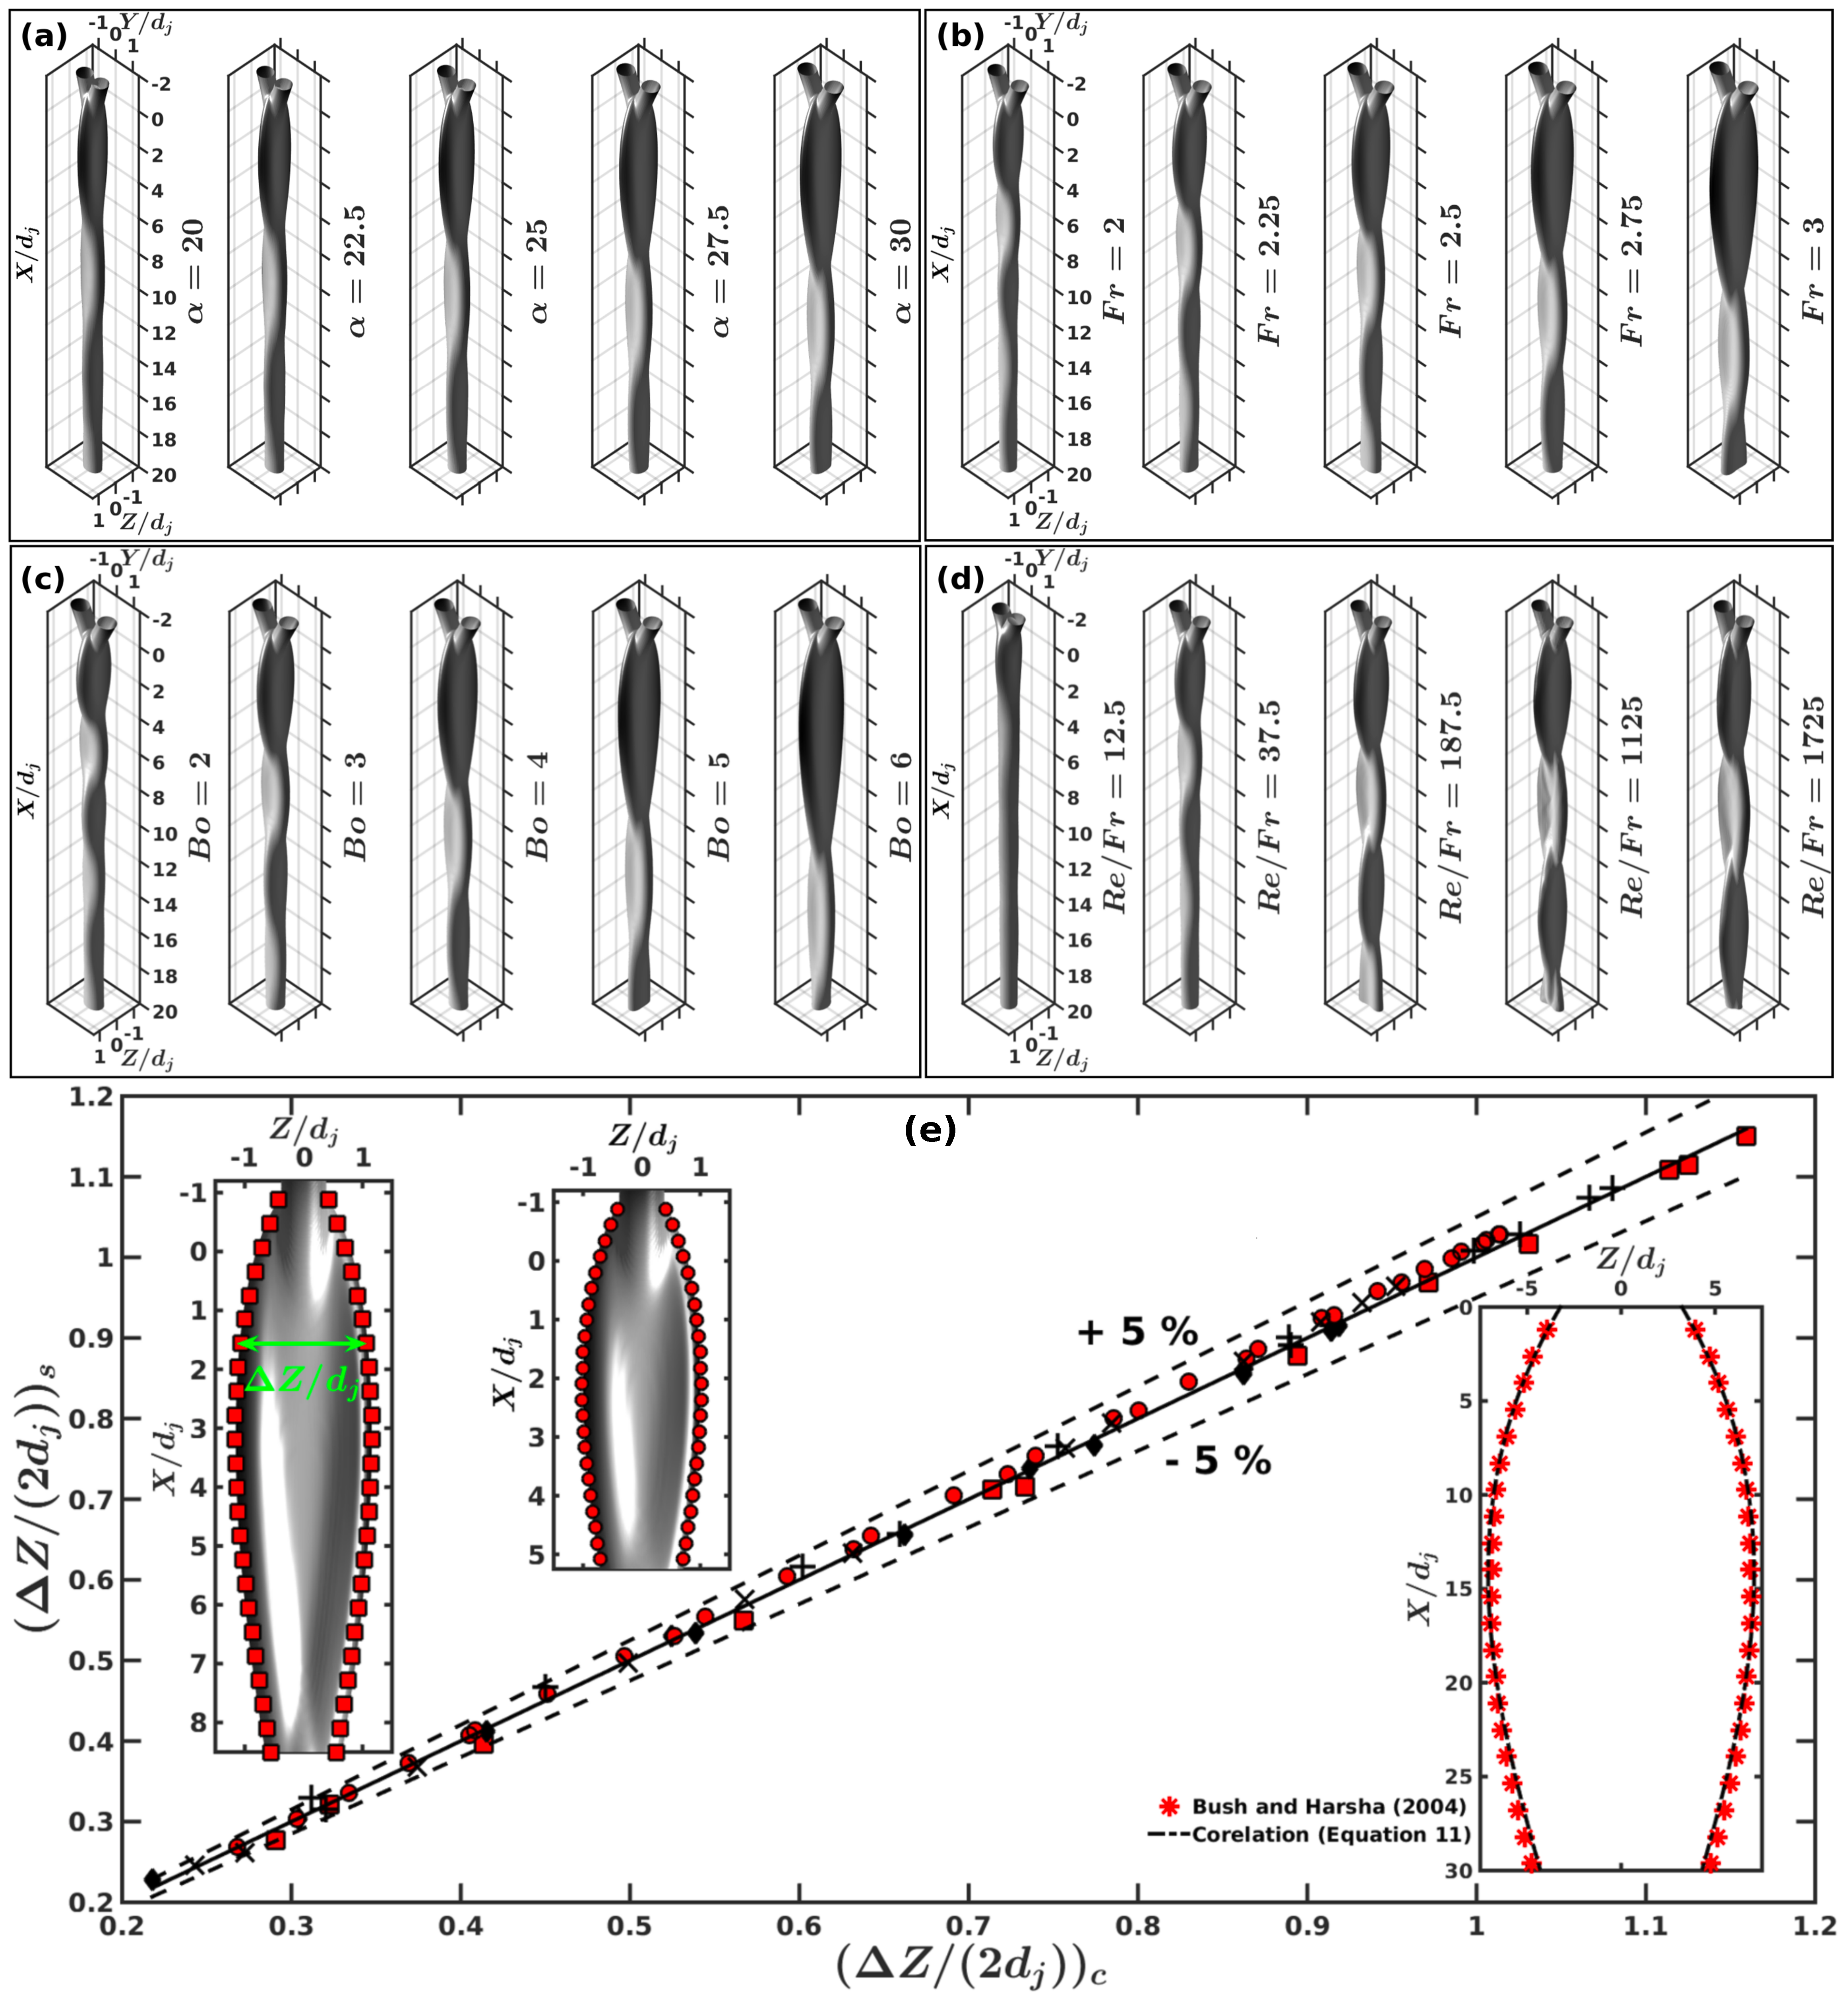
\includegraphics[width=\linewidth]{Figure6}
	\caption{High fidelity numerical simulations of liquid jets collision to form chain structure for variation of (a) $\alpha$ at $Re/Fr$ = 34,$Fr$ = 2.5, $Bo$ = 4.57, (b) $Fr$ at $Re/Fr$ = 34,$Bo$ = 3.4, $\alpha$ =  30 (c) $Bo$ at $Re/Fr$ = 34,$Fr$ = 2.5, $\alpha$ = 30, (d)  $Re/Fr$ at $Fr$ = 2,$Bo$ = 3.4, $\alpha$ = 30 and (e) Comparison between the values of expansion of the sheet outer periphery $\left(\Delta Z(x)\right)$ as predicted from equation~\ref{Equation::correlation} and from numerical simulations for different test cases with (symbol, $\alpha$, $Fr$, $Re/Fr$, $Bo$) = (\protect\MarkerSquareRed, 30$\degree$, 2.5, 34, 5); (+, 30$\degree$, 2.5, 34, 4); (\protect \MarkerDiamondBlack, 30$\degree$, 2.5, 20, 2.3); ($\times$, 25$\degree$, 2.5, 34, 4.57) and (\protect \MarkerCircleRed, 30$\degree$, 2.5, 20, 3.75).}
	\label{Figure::phaseContours}%\vspace{-3mm}
\end{figure}
Formation of the liquid sheet bounded by the rims is governed by inertia, viscous, buoyancy and surface forces apart from the angle of impingement between the jets ($\alpha$). The combination of these forces forms three non-dimensional numbers ($Fr$, $Bo$ and $Re/Fr$), described above. In this section, critical assessment of chain shapes is investigated for various non-dimensional numbers and impingement angles. \cite{yang2014liquid} acknowledged the importance of these parametric variations on collision process and formation of the first link. Figures~\ref{Figure::phaseContours}a -~\ref{Figure::phaseContours}d show numerical chain structure for a diversity of $\alpha$, $Fr$, $Bo$ and $Re/Fr$. An increase in impingement angle leads to decrement in jet momentum in direction of gravity ($u_j\cos\alpha$) and that perpendicular to the median plane increases, leading to substantial increase in width of the sheet, keeping the length more or less intact (figures~\ref{Figure::phaseContours}(a)). Alternatively, as the jet momentum is increased (increase in $Fr$), the resulting links formed are bigger (figure~\ref{Figure::phaseContours}(b)) accommodating expansion tendencies due to fluid inertia. One can clearly see this effect is transmitted to the subsequent links as well. Further, surface tension is an important entity which keeps a check on the expansion tendencies of the link. As the surface tension is decreased ($Bo$ increased), the link can expand until inertial and centrifugal forces balance it. This justifies obtaining larger links for higher values of $Bo$ as seen in figures~\ref{Figure::phaseContours}(c). As the surface tension is increased keeping all other parameters constant (low $Bo$ regime), the system tries to go towards the minimum surface energy decreasing the dimensions of the corresponding links (link in figure~\ref{Figure::phaseContours}(c) from $Bo$ = 6 to 1). Further, the collision of cylindrical jets and rims is also observed to be influenced by viscous dissipations. Keeping all other parameters constant, decreasing the viscosity (increasing $Re/Fr$) leads to considerable increase in sheet dimensions but its effect saturates at lower ranges of liquid viscosities (figure~\ref{Figure::phaseContours}(d)). Effect of change in liquid viscosity dies down as inertia and surface tension overshadows its resistance to form similar shape and sizes of links. It can also be noticed that it is the viscous dissipations that result in the decrement in the size of subsequent links leading to a point where the sheet loses its identity, giving rise to a single jet of fluid. The effect is prominent in figure~\ref{Figure::phaseContours}(d) for $Re/Fr$ = 12.5.\\
%\begin{table}
%	\centering
%	\begin{tabular}{@{}cccccc@{}}
%		&&&n&&\\
%		&$C_{m,n}$&0&1&2&3 \\
%		&0&~3.662&~2.720&~0.353&~0.512\\
%		&1&-0.082&~0.490&~1.146&~0.592\\
%		m&2&-2.166&-0.940&~0.408&~0.761\\
%		&3&-1.504&-0.831&~0.074&-0.065\\
%		&4&-0.657&-0.290&~0.029&~0.039\\
%	\end{tabular}
%\end{table} 
Considering $\Delta Z$ is the rim to rim distance at a particular vertical location ($X$) of the symmetric sheet, a third order polynomial is used to fit ($R^2$ > 0.975; $SSE$ < 0.01) the sheet shape for various influencing parameters. The functional form of the polynomial is as follows: 
\begin{equation}\label{Equation::correlation}
\frac{\Delta Z}{2d_j} = \sum_{n = 0}^{n = 3}p_n\left(\frac{X}{d_j}\right)^n
\end{equation}
Efforts are also made to relate polynomial coefficients $\left(p_n\right)$ with non-dimensional numbers using linear Regression analysis. Hence, $p_n$ can be expressed as
\begin{equation}\label{Equation::CorelationCoefficeints}
p_n = C_{0,n}\left(\sin\alpha\right)^{C_{1,n}}\left(Fr\right)^{C_{2,n}}\left(Bo\right)^{C_{3,n}}\left(Re\right)^{C_{4,n}}
\end{equation}
Values of $C_{m,n}$ in equation~\ref{Equation::CorelationCoefficeints} are tabulated in the inset of figure~\ref{Figure::phaseContours}(e) obeying $R^2$ norm of regression higher than 0.925. Predictability of the correlation with numerical chain contours are shown in the insets of figure~\ref{Figure::phaseContours}(e) for two different cases of non-dimensional numbers. It can be also observed from figure~\ref{Figure::phaseContours}(e) that developed correlation gives a very good match ($\pm$5\%) with the numerical sheet profiles. So as to check the capability of the correlation, for prediction of experimental profiles of the chain structure, the comparison is made between observation of \cite{bush2004collision} and equation~\ref{Equation::correlation}. The reported excellent match in the inset of figure~\ref{Figure::phaseContours}(e) proves the universality of the developed correlation. It is essential to understand the formation physics of widely influenced sheet structure generated due to the collision of jets. Next section dedicatedly discusses the issue.
%\vspace{-4.25mm}
\section{Analogy of chain formation}	
\begin{figure}%
	\centering
	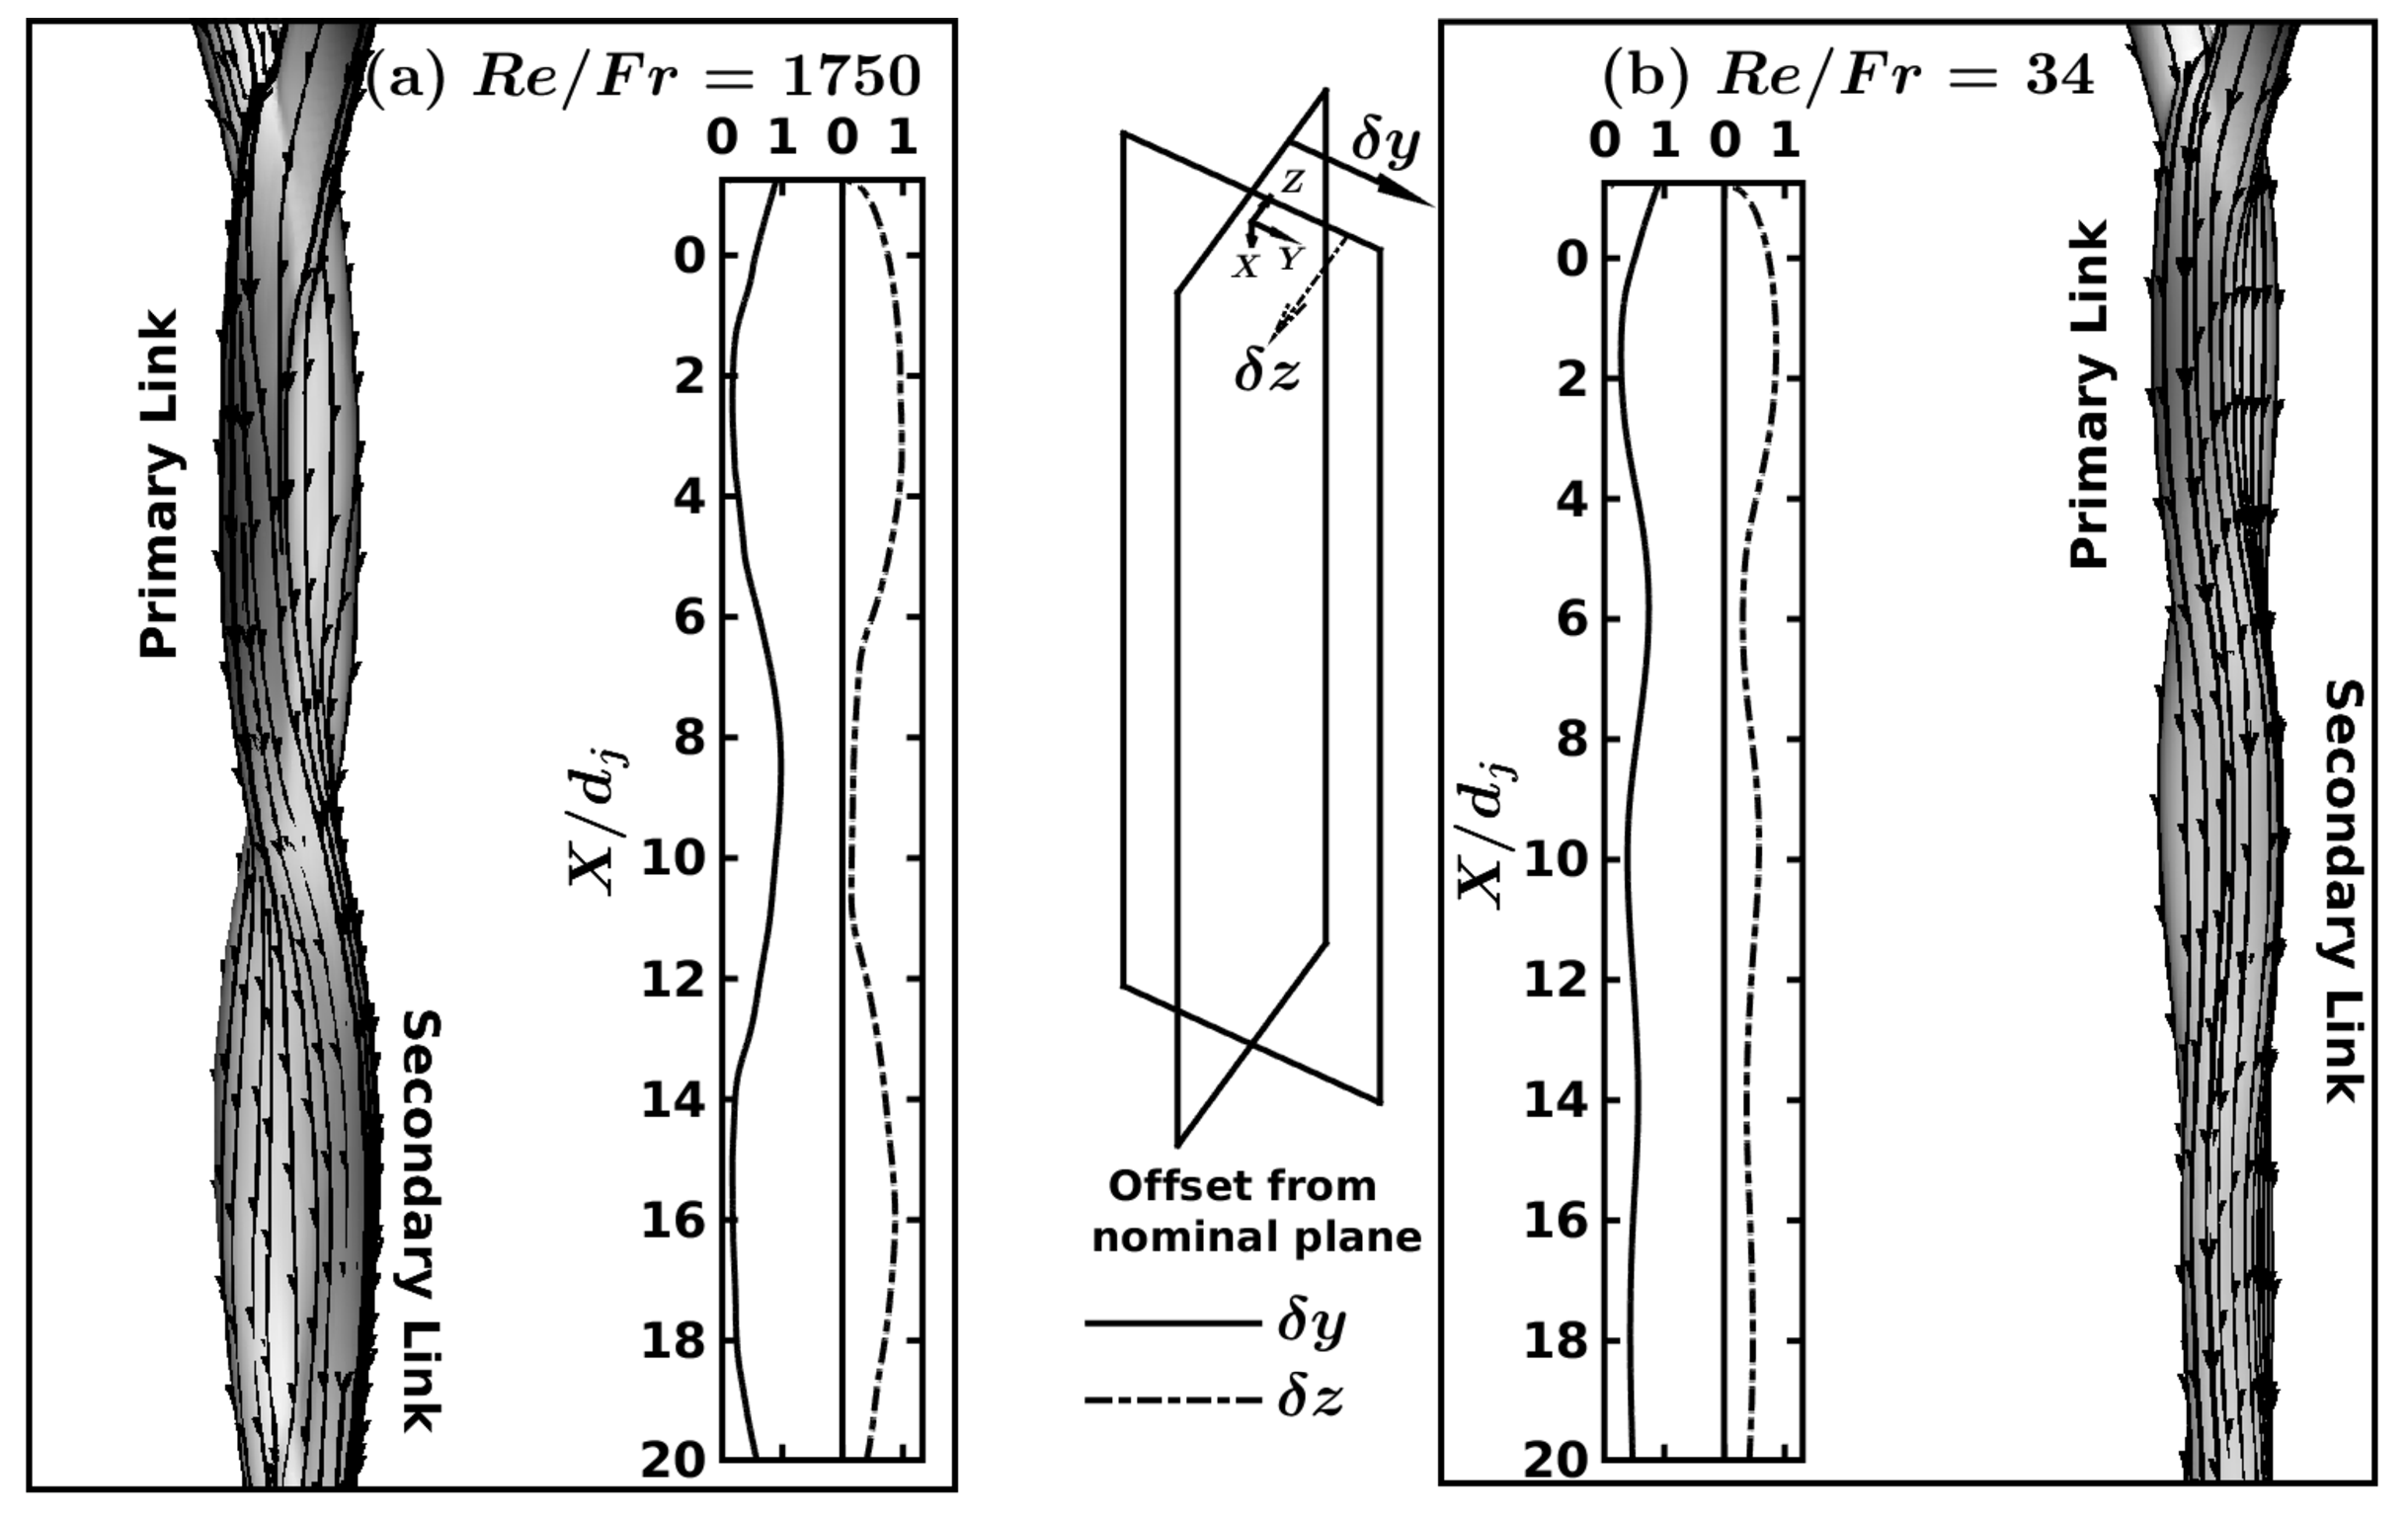
\includegraphics[width=0.75\linewidth]{Figure7}
	\caption{Billiard ball collision analogy: (a) Schematic of the model and free-body diagram and Comparison between the link shape obtained through numerical simulations and the billiard ball trajectory ($\zeta$, \protect\MarkerSquareRed) for ($\alpha$, $Fr$, $Re/Fr$, $Bo$) = (a) (30$\degree$, 2.5, 34, 5), (b) (30$\degree$, 2.5, 23, 3.85), (d) (30$\degree$, 2, 34, 4.56) and (e) (45$\degree$, 2, 34, 3.4).}
	\label{Figure::analytical}
\end{figure}%
To understand the physical insights of the liquid jet collision, idealizations are made for tracing back the sheet profile as a resultant of collision between two billiard balls (mass $m$) in the plane of the sheet. The follow-up trajectory of the balls after the collision is considered damped so as to mimic resistive forces like viscous and surface tension. A free body diagram and schematic of the billiard ball collision assumption to replicate the sheet structure is depicted in figure~\ref{Figure::analytical}(a). Apart from inertial and gravitational forces, on the ball, a damping force of magnitude $f_n$ is also attached in the direction perpendicular to the individual ball instantaneous velocity, post collision. Use of $f_n$ is supposed to impose the effect of viscous dissipation and surface forces. Absence of these resistive forces will make infinitely stretched sheet \citep{taylor1960formation}, with $f_n$ = 0 case. Reference frame for the trajectory of the ball ($\zeta$) is considered to have origin at point of collision with $\zeta$ = 0 at $X$ = 0. Free body force analysis of the ball, post-collision can be expressed as equation~\ref{Equation::forceBal}, with accelerations $a_n$ and $a_t$ in normal and tangential directions respectively.
\begin{subequations}%
	\label{Equation::forceBal}	
	\begin{eqnarray}
	\label{Equation::tangential(a)}
	\text{Direction t:}\:\:\: a_t = v_{ball}\frac{dv_{ball}}{ds} &=& g\cos\phi\\
	\text{Direction n:}\:\:\: a_n = g\sin\phi + \frac{f_n}{m} &=& \frac{v_{ball}^2}{r_c}
	\end{eqnarray}
\end{subequations}
Here, $r_c$ is the radius of curvature in $\zeta-X$ plane and $\phi = \tan^{-1}\left(\frac{d\zeta}{dX}\right)$. Integrating tangential momentum equation with increment $ds = dX/\cos\phi$ along with boundary condition at $X$ = 0, instantaneous ball velocity ($v_{ball}$) can be obtained as $\sqrt{u_j^2 + 2gX}$. Rearrangement of momentum equation in the normal direction after defining $\Lambda$ as $\frac{f_n}{mg}$ and inertial length scale, $\chi$ equivalent to $\frac{u_j^2}{2g}$, one obtains:
\begin{equation}\label{Equation::Final1}
r_c\left(\sin\phi + \Lambda\right) = 2\chi\left(\frac{X}{\chi} + 1\right)
\end{equation} 
After necessary integration, equation~\ref{Equation::Final1} simplifies to:
\begin{equation}
\sin\phi  = \sin\alpha + \left(\Lambda + \sin\alpha\right)\left(\frac{1}{\sqrt{\frac{X}{\chi} + 1}} - 1\right)	
\end{equation}
Recalling that $\tan\phi = \frac{d\zeta}{dX}$ and expressing $\Lambda/\sin\alpha = \eta$, profile of billiard ball movement can be characterized as:
\begin{equation}
\label{Equation::AnaFinal}
\frac{d\zeta}{dX} = \tan\left\lbrace\sin^{-1}\left[ \sin\phi_0\left(1 + \eta\right)\left(\frac{1}{\sqrt{\frac{X}{\chi} + 1}} - 1\right) \right]\right\rbrace
\end{equation}
The functional form of the ball trajectory, equivalence of sheet profile, can be integrated numerically to obtain the coordinate points in the $\zeta-X$ plane after tuning only control factor, $\eta$ from some simulated profiles. In this process, $L^1$ relative error norm is kept below 10\%. Efforts have been also made to express control parameter, $\eta$ in terms of non-dimensional numbers for the range of values presented in this work. With 99\% $R^2$ regression norm, $\eta$ can be related with non-dimensional numbers as:
\begin{equation}\label{Equation::eta}
\eta = 3.28(\sin\alpha)^{-0.077}(Fr)^{0.502}(Bo)^{-0.248}\left(Re\right)^{-0.084}
\end{equation}
Proposed concept of collision of billiard balls for mimicking the sheet profile is also tested with phase contours of numerical simulations. Some representative matches are shown in figure~\ref{Figure::analytical}(b) -~\ref{Figure::analytical}(e) in connection of primary link. Fundamental analysis of forces, a single controlling parameter in sheet profile (equation~\ref{Equation::AnaFinal}) and an excellent match with numerical data supplies in-depth knowledge about the genesis of the liquid chain. Next, we focus on the mutual relationship between links formed at successive orthogonal planes. 
%\vspace{-4mm}
\section{Inter-relation between inter-connected links} 
\begin{figure}
	\centering
	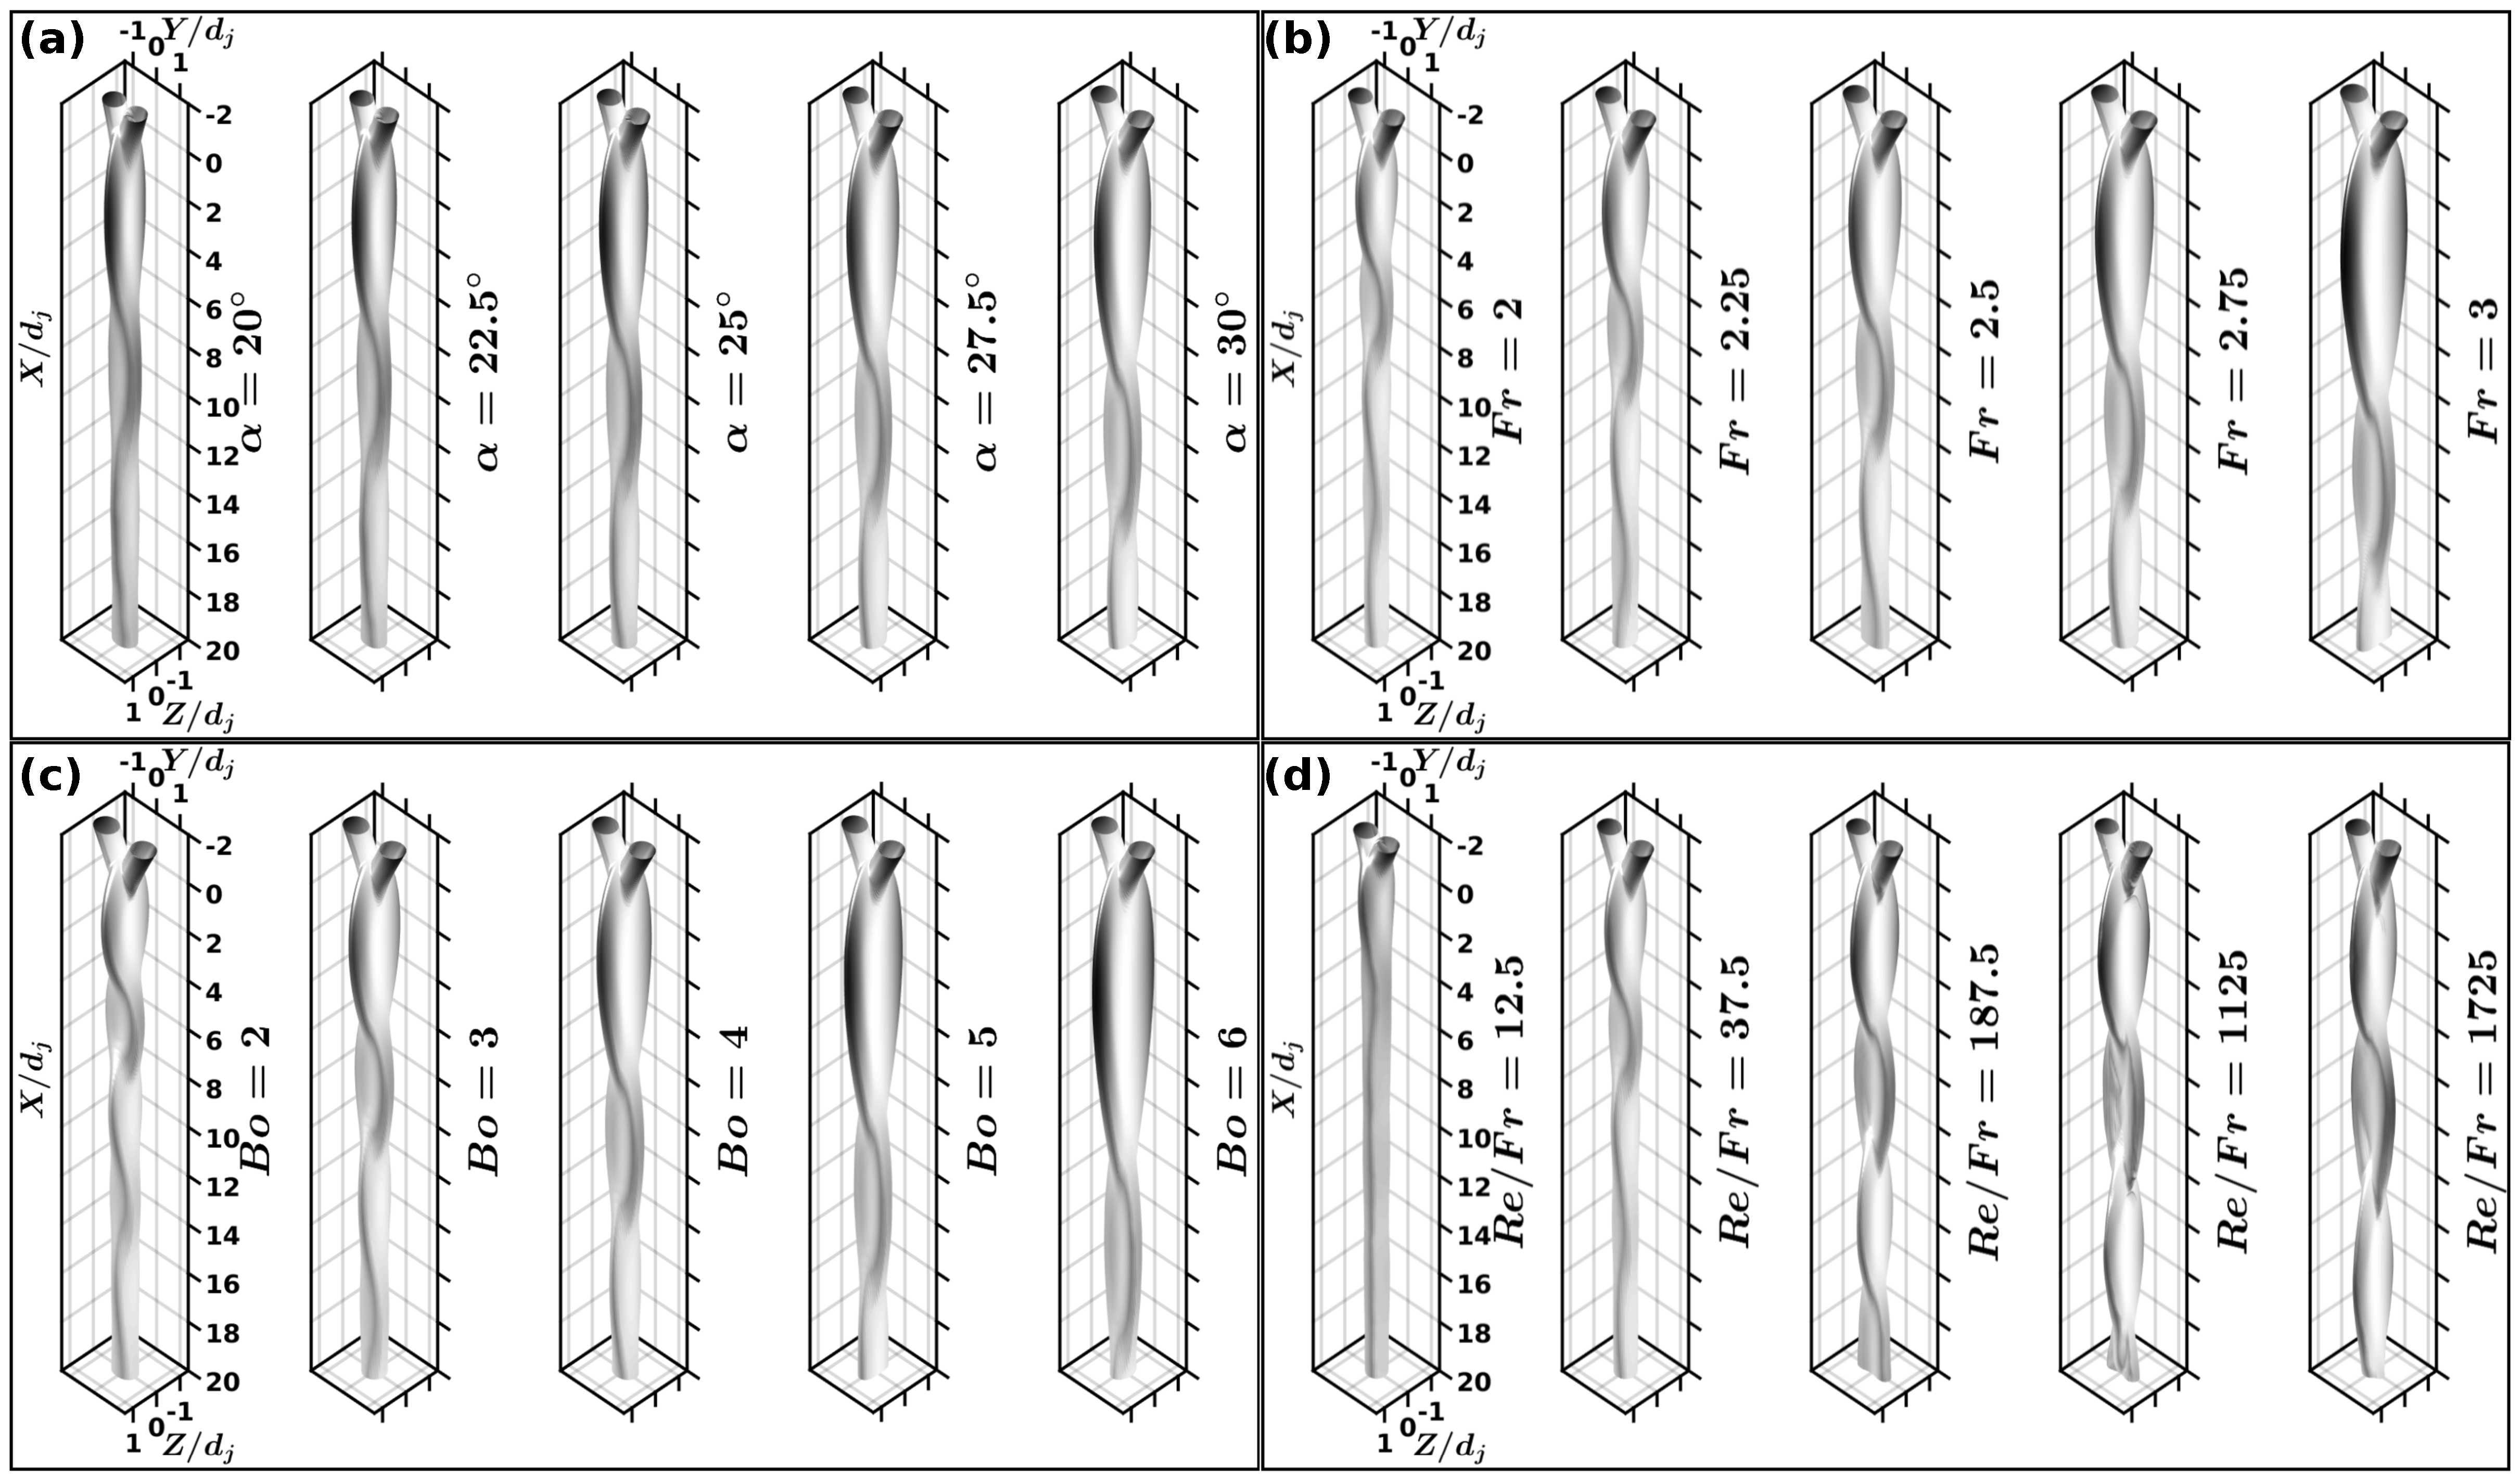
\includegraphics[width=\linewidth]{Figure8}
	\caption{Inter-relation between links of chain (a) Reproduction of secondary link of Case 1 ($\alpha$ = 30$\degree$, $Fr$ = 2.5, $Re/Fr$ = 34, $Bo$ = 4) as primary link of case 2 ($\alpha$ = 25$\degree$, $Fr$ = 2.2, $Re/Fr$ = 34, $Bo$ = 4) and tertiary link of case 1 as secondary link of case 2 and primary link of case 3 ($\alpha$ = 11.25$\degree$, $Fr$ = 1.98, $Re/Fr$ = 34, $Bo$ = 4), Prediction of angles of impingement for (b) Secondary and (c) Tertiary collision and (d) Subsequent collision $Fr$.}
	\label{Figure::secondCollision}%%\vspace{-2.5mm}
\end{figure}
The secondary and tertiary links observed in mutually perpendicular planes initiate with the collision of rims in preceding links. From our numerous simulations in the wide range of operating parameters, it can be observed that secondary, tertiary and subsequent links of a chain are equivalent to primary, secondary and subsequent links of another chain having different operating parameters. Hence, it is proposed that subsequent links are equivalent to resultant of collision between two free jets having reduced strength. To establish our claim, in figure~\ref{Figure::secondCollision}(a), a representative chain structure is identified for $\alpha$ = 30$\degree$, $Fr$ = 2.5, $Re/Fr$ = 34, $Bo$ = 4 (Case 1), in which secondary links showed resemblance with primary link of $\alpha$ = 25$\degree$, $Fr$ = 2.2, $Re/Fr$ = 34, $Bo$ = 4 (Case 2). Continuing this one can also establish analogy among tertiary link of case 1, secondary link of case 2 and primary link of $\alpha$ = 11.25$\degree$, $Fr$ = 1.98, $Re/Fr$ = 34, $Bo$ = 4 (Case 3). One to one correspondence of these links of different cases establishing present proposal is shown in the comparative graph of figure~\ref{Figure::secondCollision}(a). It can be commented that subsequent links are reduced in size, giving a feeling of resultant of impact between two lesser strength jets. The analogy of interconnected links in a chain with one level lesser link in another chain is found to be valid with $\pm$ 10\% confidence for the entire region of search space of the operating parameters ($\alpha$, $Fr$, $Re/Fr$, $Bo$). A critical assessment of links in chain structure and rim profile have also established that angle of impingement between rims successively reduces $\alpha_{n}/\alpha_{n-1} < 1 \:\:\forall\:\: n = 1, 2, 3 \:\:\text{and higher integers}$. It has been also checked that analogy of collision between billiard balls and formation of the link by the interaction between rims is also valid after taking the reduction of angle of impingement into consideration. This idea we have established in figure~\ref{Figure::secondCollision}(b) -~\ref{Figure::secondCollision}(c) for secondary and tertiary links for few chain cases randomly scattered in search space. With only $\pm$ 10\% error, theory of collision between billiard balls (equations~\ref{Equation::AnaFinal} -~\ref{Equation::eta}) has also found to be applicable for $n^{th}$ order link of chain. Polynomial proposed in equation~\ref{Equation::correlation} also predicts genesis of $n^{th}$ order link satisfactorily with modified strength and impingement angle. Clustering of points near (1,1) for secondary link (figure~\ref{Figure::secondCollision}(b)) and (0,0) for tertiary link (figure~\ref{Figure::secondCollision}(c)) establishes continuous reduction of impingement angle $\alpha_{n}$ with increase in link number $n$. Besides the reduction in angle of impingements, the interaction between rims of a link also can be considered as the collision between jets of lesser Froude number ($Fr_m$) than $Fr_j$. The monotonous decrement of $Fr_m$ is observed as one traverses in subsequent higher level links along a chain. Figure~\ref{Figure::secondCollision}(d) establishes this idea where ratio between rim Froude number of secondary link ($Fr_2$) to jet Froude number ($Fr_j$) has been fitted as 0.88 and that of same for tertiary link ($Fr_3/Fr_j$) as 0.8. Though idea of inter-relation between links is established only for first three, it can be extrapolated for higher order elements in the chain until it transforms to jet.
\section{Conclusion}
The stable chain structures are formed by the collision of laminar liquid jets when the inertia forces are, in order of magnitude, similar to the surface tension forces. Numerical simulations showed that individual links, formed by collision of cylindrical jets (primary) or rims (secondary onward), occupy mutually orthogonal planes with a successive reduction in size owing to viscous effects. The fluid parcels inside these links are dispatched radially outwards from the stagnation point and follow trajectories self-similar to the phase boundary. The inertial and gravitational forces provide a measure of the expansion of these sheets counteracted by the surface tension at the interface and viscous dissipations at the subsequent collisions. These symmetric sheet profile can be modeled using a third order polynomial, at an accuracy of $\pm$ 5\%, with coefficients dependent on various non-dimensional numbers featuring the interplay of different forces. Effects of these forces have been understood by mimicking them onto the post-collision trajectory of billiard balls. Higher order links are found to be similar to lower or primary level element formed due to impact between jets of reduced $Fr$ and $\alpha$. 
\bibliographystyle{jfm}
\bibliography{chains}
\end{document}
